%--------------------------------------------------------------------%
%
% Berkas utama templat LaTeX.
%
% author Ilham Firadusi Putra
% template dari Petra Barus dan Peb Ruswono Aryan
%
%--------------------------------------------------------------------%
%
% Berkas ini berisi struktur utama dokumen LaTeX yang akan dibuat.
%
%--------------------------------------------------------------------%

\documentclass[12pt, a4paper, onecolumn, oneside, final]{report}

%-------------------------------------------------------------------%
%
% Konfigurasi dokumen LaTeX untuk laporan tesis IF ITB
%
% @author Ilham Firdausi Putra
%
%-------------------------------------------------------------------%
%
% Berkas ini merupakan pembaharuan dari berkas awal milik Petra Novandi dan Steven Lolong
%
%-------------------------------------------------------------------%

% Ukuran kertas
\special{papersize=210mm,297mm}

% Setting margin
\usepackage[top=3cm,bottom=2.5cm,left=4cm,right=2.5cm]{geometry}

\usepackage{mathptmx}

% Format citation
\usepackage[backend=bibtex,citestyle=authoryear,sorting=nyt,firstinits=true]{biblatex}
\renewcommand*{\nameyeardelim}{\addcomma\space}
\renewcommand*\finalnamedelim{\addspace\&\space}

% Anti hyphenation
\tolerance=1
\emergencystretch=\maxdimen
\hyphenpenalty=10000
\hbadness=10000

% Judul bahasa Indonesia
\usepackage[russian, bahasa]{babel}
\usepackage[utf8]{inputenc}
\usepackage{csquotes}
\setquotestyle{english}
\usepackage{graphicx}
\usepackage{titling}
\usepackage{blindtext}
\usepackage{sectsty}
\usepackage{chngcntr}
\usepackage{etoolbox}
\usepackage{hyperref}       % Package untuk link di daftar isi.
\usepackage{titlesec}       % Package Format judul
\usepackage{parskip}

% Daftar Istilah
\usepackage{tabularx}

% confusion matrix
\usepackage{multirow}

% package di equation
\usepackage{amsmath}
\usepackage{amsfonts}

% Line satu setengah spasi
\renewcommand{\baselinestretch}{1.5}

% Setting judul chapter
\chapterfont{\centering \large}
\titleformat{\chapter}[display]
  {\large\centering\bfseries}
  {\chaptertitlename\ \thechapter}{0pt}
    {\large\bfseries\uppercase}

\titlespacing*{\chapter}{0pt}{-30pt}{40pt}
\titlespacing*{\section}{0pt}{10pt}{0pt}
\titlespacing*{\subsection}{0pt}{10pt}{0pt}

% Setting besar font section
% \newcommand{\secfnt}{\fontsize{8}{12}}
% \newcommand{\ssecfnt}{\fontsize{8}{12}}

% \titleformat{\section}
% {\normalfont\secfnt\bfseries}{\thesection}{1em}{}

% \titleformat{\subsection}
% {\normalfont\ssecfnt\bfseries}{\thesubsection}{1em}{}
% \titleformat*{\section}{\normalsize\bfseries}
% \titleformat*{\subsection}{\normalsize\bfseries}
% \sectionfont{\fontsize{8}{12}\selectfont}

% Untuk nampilin kode
\usepackage[utf8]{inputenc}
 
\usepackage{listings}
\usepackage{xcolor}
 
\definecolor{codegreen}{rgb}{0,0.6,0}
\definecolor{codegray}{rgb}{0.5,0.5,0.5}
\definecolor{codepurple}{rgb}{0.58,0,0.82}
\definecolor{backcolour}{rgb}{0.95,0.95,0.92}
 
\lstdefinestyle{mystyle}{
    backgroundcolor=\color{backcolour},   
    commentstyle=\color{codegreen},
    keywordstyle=\color{magenta},
    numberstyle=\tiny\color{codegray},
    stringstyle=\color{codepurple},
    basicstyle=\ttfamily\footnotesize,
    breakatwhitespace=false,         
    breaklines=true,                 
    captionpos=b,                    
    keepspaces=true,                 
    numbers=left,                    
    numbersep=5pt,                  
    showspaces=false,                
    showstringspaces=false,
    showtabs=false,                  
    tabsize=2
}
 
\lstset{style=mystyle}

% Setting nomor pada subbsubsubbab
\setcounter{secnumdepth}{3}

\makeatletter

\makeatother

% Counter untuk figure dan table.
\counterwithin{figure}{section}
\counterwithin{table}{section}

% bahasa asing
\usepackage{CJKutf8}

% Spacing pada daftar figure dan table
\makeatletter
     \renewcommand*\l@figure{\@dottedtocline{1}{1em}{3.2em}}
\makeatother

\makeatletter
     \renewcommand*\l@table{\@dottedtocline{1}{1em}{3.2em}}
\makeatother


% Ganti judul bibliography
% \renewcommand\bibname{Daftar Pustaka}


\makeatletter

\makeatother

\bibliography{references}

\begin{document}

    %Basic configuration
    \title{Klasifikasi Teks Berbahasa Indonesia Menggunakan \textit{Multi-lingual Language Model}}
    \date{}
    \author{
        Ilham Firdausi Putra\\
        NIM 13516140
    }

    \pagenumbering{roman}
    \setcounter{page}{0}

    \clearpage
\pagestyle{empty}

\begin{center}
\smallskip

    \Large \bfseries \MakeUppercase{\thetitle}
    \vfill

    \Large Laporan Tugas Akhir 2
    \vfill

    \large Disusun sebagai syarat kelulusan tingkat sarjana
    \vfill

    \large Oleh

    \Large \theauthor

    \vfill
    \begin{figure}[h]
        \centering
      	
\includegraphics[width=0.2\textwidth]{resources/cover-ganesha.jpg}
    \end{figure}
    \vfill

    \large
    \uppercase{
        Program Studi Teknik Informatika \\
        Sekolah Teknik Elektro dan Informatika \\
        Institut Teknologi Bandung
    }

    April 2020

\end{center}

\clearpage

    \clearpage
\pagestyle{empty}

\begin{center}
\smallskip

    \Large \bfseries \MakeUppercase{\thetitle}
    \vfill

    \Large Laporan Tugas Akhir
    \vfill

    \large Oleh

    \Large \theauthor

    \large Program Studi Teknik Informatika \\
    Sekolah Teknik Elektro dan Informatika \\
    Institut Teknologi Bandung \\

    \vfill
    \normalsize \normalfont
    Telah disetujui dan disahkan sebagai Laporan Tugas Akhir 2 di Bandung, pada tanggal 5 Mei 2020.

    \vfill
    \normalsize \normalfont
    Pembimbing\\
    ~\\
    ~\\
    ~\\
    ~\\
    \underline{Dr. Eng. Ayu Purwarianti, ST.,MT.} \\
    NIP 19770127 200801 2 011

    % \begin{tabular}{c@{\hskip 0.5in}c}
    %     Pembimbing I, & Pembimbing II \\
    %     & \\
    %     & \\
    %     & \\
    %     & \\
    %     Dr. Eng. Ayu Purwarianti, ST.,MT. & Nama dan Gelar Pembimbing II \\
    %     NIP 19770127 200801 2 011 & NIP 123456789 \\
    % \end{tabular}

\end{center}
\clearpage

    \clearpage

\chapter*{Lembar Pernyataan}

Dengan ini saya menyatakan bahwa:

\begin{enumerate}

    \item Pengerjaan dan penulisan Laporan Tugas Akhir ini dilakukan tanpa menggunakan bantuan yang tidak dibenarkan.
    \item Segala bentuk kutipan dan acuan terhadap tulisan orang lain yang digunakan di dalam penyusunan laporan tugas akhir ini telah dituliskan dengan baik dan benar.
    \item Laporan Tugas Akhir ini belum pernah diajukan pada program pendidikan di perguruan tinggi mana pun.

\end{enumerate}

Jika terbukti melanggar hal-hal di atas, saya bersedia dikenakan sanksi sesuai dengan Peraturan Akademik dan Kemahasiswaan Institut Teknologi Bandung bagian Penegakan Norma Akademik dan Kemahasiswaan khususnya Pasal 2.1 dan Pasal 2.2.
\vspace{15mm}



\begin{flushright} 
    Bandung, 22 Juni 2020 \\
    \vskip 0.5in
    % \begin{figure}[!h]
    %     \raggedleft
    %     
\includegraphics[width=0.2\textwidth]{resources/tandatangan.png}
    % \end{figure}
    Ilham Firdausi Putra \\
    NIM 13516140
\end{flushright}

\clearpage

    \pagestyle{plain}

    % \clearpage
\chapter*{ABSTRAK}
\addcontentsline{toc}{chapter}{Abstrak}
\begin{center} 
    \large \bfseries \MakeUppercase{Klasifikasi Teks Berbahasa Indonesia Menggunakan \textit{Multilingual Language Model (Studi Kasus: Klasifikasi Ujaran Kebencian dan Analisis Sentimen)}} 

    \normalsize \normalfont{Oleh\\
    ILHAM FIRDAUSI PUTRA\\
    NIM : 13516140
    }
\end{center}

%taruh abstrak bahasa indonesia di sini

Klasifikasi teks adalah proses memprediksi kategori tertentu dari sebuah teks. Contoh kategori adalah nilai sentimen atau status ujaran kebencian. Teknik klasifikasi teks \textit{state-of-the-art} saat ini menggunakan deep learning yang memerlukan data latih dalam ukuran besar. Bersamaan dengan itu, perkembangan dalam bidang representasi teks telah memungkinkan teks dari berbagai bahasa direpresentasikan dalam satu bidang yang sama menggunakan \textit{multilingual language model}. Dua diantaranya adalah MultilingualBERT \parencite{Devlin_Chang_Lee_Toutanova_2019} dan XLM-R\parencite{Conneau_XLMR}.

Dengan memanfaatkan MultilingualBERT dan XLM-R, representasi teks antar bahasa dapat digunakan untuk membangun model klasifikasi bahasa Indonesia dengan kombinasi data bahasa Indonesia dan bahasa Inggris. Tugas akhir ini memanfaatkan hal tersebut untuk membangun model klasifikasi teks bahasa Indonesia yang meningkatkan performa hasil penelitian \parencite{FarhanKhodra2017} \& \parencite{CrisdayantiPurwarianti2019} mengenai analisis sentimen dan versi biner penelitian \parencite{Ibrohim_Budi_2019} mengenai ujaran kebencian \& kasar. Eksperimen dilakukan dengan memvariasikan jumlah data bahasa Indonesia, jumlah data bahasa Inggris, dan teknik \textit{fine-tuning}.

Hasil eksperimen menunjukkan XLM-R berhasil meningkat hasil analisis sentimen pada dataset penelitian \parencite{FarhanKhodra2017} dari F1-score 0,8341 ke 0,893; penelitian \parencite{CrisdayantiPurwarianti2019} dari F1-score 0,9369 ke 1; dan penelitian \parencite{Ibrohim_Budi_2019} dari rata-rata akurasi 77.36\% ke 89.52\%. Meski ada kasus dimana penambahan data bahasa Inggris berlebih menurunkan performa klasifikasi yang harus dianalisa lebih lanjut, hasil eksperimen menunjukkan bahwa penambahan dataset bahasa Inggris, terutama jika data bahasa Indonesia sedikit, dapat membantu meningkatkan performa klasifikasi teks bahasa Indonesia menggunakan model XLM-R.

\textbf{Kata kunci:} \textit{multilingual language model}, analisis sentimen, klasifikasi ujaran kebencian
\clearpage
    % \clearpage
\chapter*{Abstract}
\addcontentsline{toc}{chapter}{Abstract}

%put your abstract here
\blindtext

\clearpage
    % \chapter*{Kata Pengantar}
\addcontentsline{toc}{chapter}{Kata Pengantar}

Puji syukur penulis panjatkan ke hadirat Tuhan Yang Maha Kuasa karena atas berkat dan karunia-Nya, penulis dapat menyelesaikan tugas akhir yang berjudul “Klasifikasi Teks Berbahasa Indonesia Menggunakan \textit{Multilingual Language Model (Studi Kasus: Klasifikasi Ujaran Kebencian dan Analisis Sentimen)}” untuk memenuhi syarat kelulusan tingkat sarjana. Penulis juga ingin mengucapkan terima kasih kepada pihak-pihak yang telah membantu dan mendukung penulis selama pengerjaan tugas akhir ini:

\begin{enumerate}
    \item Ibu Dr. Eng. Ayu Purwarianti, ST.,MT., selaku dosen pembimbing yang telah memberikan arahan, nasehat, dan dukungan selama pengerjaan tugas akhir.
    \item Ibu Fariska Zakhralativa Ruskanda S.T., M.T., dan Ibu Dr. Masayu Leylia Khodra, ST., MT. selaku dosen penguji yang telah memberikan evaluasi dan saran kepada penulis.
    \item Ibu Dessi Puji Lestari S.T.,M.Eng.,Ph.D, Ibu Dr. Fazat Nur Azizah S.T., M.Sc., dan Bapak Nugraha Priya Utama, Ph.D. selaku dosen mata kuliah IF4091 Tugas Akhir I K01 dan IF4092 Tugas Akhir II yang telah memberi arahan selama pelaksanaan tugas akhir ini.
    \item Ibu Dra. Harlili M.Sc. selaku dosen wali yang telah memberikan arahan, nasehat, dan dukungan selama empat tahun berkuliah di program studi Teknik Informatika ITB.
    \item Keluarga penulis yang selalu mendukung dan memotivasi penulis untuk tetap semangat dalam kuliah hingga menyelesaikan tugas akhir.
    \item Seluruh staf pengajar yang belum disebutkan dari program studi Teknik Informatika yang telah membekali penulis dengan ilmu dan wawasan untuk mendukung pengerjaan tugas akhir.
    \item Staf Tata Usaha program studi Teknik Informatika yang telah membantu selama perkuliahan khususnya dalam proses administrasi tugas akhir.
    \item Teman-teman penulis yang telah mendukung serta menemani perjalanan kuliah dan pengerjaan tugas akhir ini.

    
\end{enumerate}
Akhir kata, terima kasih banyak kepada semua pihak yang telah secara langsung maupun tidak langsung membantu penyelesaian tugas akhir ini. Penulis berharap tugas akhir ini dapat bermanfaat bagi para pembaca. Penulis juga menyadari bahwa tugas akhir ini tidaklah sempurna. Oleh karena itu, penulis sangat terbuka terhadap kritik dan saran yang membangun terkait tugas akhir ini.

\begin{flushright} 
    Bandung, 22 Juni 2020 \\
    % \begin{figure}[!h]
    %     \raggedleft
    %     
\includegraphics[width=0.2\textwidth]{resources/tandatangan.png}
    % \end{figure}
    Penulis
\end{flushright}
\clearpage


    % \titleformat*{\section}{\centering\bfseries\Large\MakeUpperCase}
    \titleformat*{\section}{\centering\bfseries\fontsize{8}{12}\MakeUpperCase}

    \tableofcontents
    \listoffigures
    \listoftables

    % \titleformat*{\section}{\bfseries\Large}
    \titleformat*{\section}{\bfseries\fontsize{8}{12}}
    \titleformat*{\subsection}{\bfseries\fontsize{8}{12}}
    \pagenumbering{arabic}

    %----------------------------------------------------------------%
    % Konfigurasi Bab
    %----------------------------------------------------------------%
    \setcounter{page}{0}
    \renewcommand{\chaptername}{BAB}
    \renewcommand{\thechapter}{\Roman{chapter}}
    %----------------------------------------------------------------%

    %----------------------------------------------------------------%
    % Dafter Bab
    % Untuk menambahkan daftar bab, buat berkas bab misalnya `chapter-6` di direktori `chapters`, dan masukkan ke sini.
    %----------------------------------------------------------------%
    \chapter{Pendahuluan}

Bab pendahuluan ini menjelaskan tentang landasan pembuatan tugas akhir mengenai klasifikasi teks berbahasa Indonesia menggunakan \textit{multilingual language model}. Bab ini terdiri dari latar belakang, rumusan masalah, tujuan, batasan masalah, metodologi, dan jadwal pelaksanaan tugas akhir.

\section{Latar Belakang}

Permasalahan klasifikasi pembelajaran mesin \textit{supervised} dapat digambarkan sebagai berikut: diberikan satu set label klasifikasi C, dan satu set contoh pelatihan E, yang masing-masing telah diberi salah satu label kelas dari C, sistem harus menggunakan contoh pelatihan E untuk membentuk hipotesis yang dapat digunakan untuk memprediksi label kelas dari contoh baru yang tak digunakan untuk melatih \parencite{mitchell_machine_1997}. Dalam permasalahan klasifikasi teks, data pelatihan E merupakan teks seperti dokumen atau komentar daring pada media sosial. Sedangkan label dapat berupa topik, judul, atau informasi lainnya yang dapat diambil dari teks.

Sebelum sebuah teks dapat diproses, algoritma pembelajaran mesin memerlukan representasi teks dalam bentuk numerik. Untuk hal itu, berkembanglah berbagai teknik untuk merepresentasikan teks sebaik mungkin. Bentuk paling sederhananya adalah pendekatan \textit{one-hot-vector} yang merepresentasikan teks berdasarkan ada atau tidaknya saja. Representasi seperti ini memiliki kekurangan seperti tidak diperhatikannya letak kata dan membesarnya representasi kata seiring membesarnya kosa kata. Kekurangan ini dapat diselesaikan dengan \textit{word embedding} seperti Word2vec \parencite{MikolovWord2vec} yang mempelajari representasi kata sebagai vektor bernilai riil. Tetapi kelemahan pemrosesan teks dengan \textit{word embedding} adalah masih dangkalnya representasi. Representasi \textit{word embedding} tidak dapat menangkap interaksi antar kata di kalimat yang kompleks. Oleh karena itu, berkembanglah \textit{language model} seperti BERT \parencite{Devlin_Chang_Lee_Toutanova_2019} dan XLM \parencite{LampleConneau2019} yang tidak hanya belajar di level kata, tetapi sampai dapat memperhatikan konteks di mana kata tersebut berada. 

Pengembangan representasi teks yang akurat memerlukan banyak data teks. Bahasa Indonesia sebagai bahasa yang ingin diteliti di sini memiliki lebih sedikit data teks dibanding bahasa yang lebih populer seperti bahasa Inggris. Sebagai contoh, pada permasalahan analisis sentimen dan ujarna kebencian, bahasa Inggris memiliki dataset seperti \textit{Yelp Review}\footnote{\url{https://www.yelp.com/dataset/challenge}} dan \textit{Jigsaw Toxic Comment}\footnote{\url{https://www.kaggle.com/c/jigsaw-unintended-bias-in-toxicity-classificationl}} yang totalnya hingga jutaan data. 

Perkembangan dalam bidang representasi teks telah memungkinkan teks dari berbagai bahasa direpresentasikan dalam satu bidang yang sama. Untuk menanggulangi masalah kurangnya data, representasi teks antar bahasa dapat dimanfaatkan untuk membangun model klasifikasi bahasa Indonesia dengan menggunakan kombinasi data bahasa Indonesia dan bahasa lain. Suatu teknik yang memperhitungkan semua dokumen pelatihan dari semua bahasa ketika membangun model klasifikasi \textit{monolingual} untuk bahasa tertentu sudah didemonstrasikan oleh \parencite{Wei_Shi_Yang_2007}. Pada demonstrasinya, mereka menunjukkan bahwa pendekatan ini lebih akurat dibanding model yang hanya dilatih pada satu bahasa saja untuk permasalahan kategorisasi teks. 

% Transfer Learning adalah teknik melakukan pembelajaran mesin dari sebuah domain, biasanya yang memiliki lebih banyak data, lalu menggunakan model yang sudah dipelajari untuk menyelesaikan masalah di domain lainnya \parencite{ruder2019transfer}. Penggunaan teknik ini sangat sukses mendorong kemajuan besar di berbagai permasalahan pemrosesan teks alami. Dengan transfer learning lintas bahasa, bahasa yang memiliki sumber daya rendah dapat memanfaatkan sumber daya dari bahasa yang jauh lebih kaya.

Dengan berkembangnya akses masyarakat Indonesia ke internet, semakin banyak data teks yang tersedia secara digital. Data ini penuh informasi dan sangat berguna jika diolah. Bagi pemilik bisnis contohnya, komentar warganet di internet dapat dianalisis sentimennya untuk mengetahui reaksi mereka terhadap sesuatu. Lalu bagi yang memiliki website, mendeteksi pelanggaran dalam percakapan online seperti ujaran kebencian atau kasar secara otomatis dapat sangat membantu. Permasalahan analisis sentimen dan klasifikasi ujaran kebencian \& kasar tersebutlah yang akan menjadi fokus dalam tugas akhir ini.

Analisis sentimen adalah proses pendeteksian dan pengekstraksian informasi subjektif mengenai sentimen dalam sebuah teks. Hal ini dapat dilakukan pada beberapa level ekstraksi yaitu pada level dokumen, kalimat, hingga level spesifik terkait aspek tertentu \parencite{Liu2012}. Pada level paling granular, analisis sentimen dilakukan pada level aspek. Pada level kalimat, sentimen ditentukan untuk setiap kalimat meskipun dalam satu kalimat dapat memiliki lebih dari satu aspek. Dan terakhir pada level dokumen, analisis sentimen dilakukan secara keseluruhan meskipun dalam satu dokumen dapat memiliki lebih dari satu kalimat dan aspek sentimen. Meski analisis sentimen pada level lebih granular dapat memberikan analisa lebih detail, analisis sentimen pada level dokumen masih banyak digunakan untuk mengetahui sentimen secara keseluruhan.

Klasifikasi ujaran kebencian \& kasar adalah proses mengategorikan sebuah teks, biasanya komentar di sosial media atau web, berdasarkan masuk atau tidaknya teks tersebut dalam definisi ujaran yang mengandung kebencian \& kasar. Hal ini dapat dilakukan secara biner dan multi-kelas / multi-label. Pada kasus biner, teks hanya dikategorikan sebagai ujaran yang mengandung kebencian \& kasar atau tidak mengandung sama sekali. Sedangkan pada kasus multi-kelas / multi-label, teks selanjutnya dianalisa untuk mengetahui siapa targetnya atau seberapa parah ujaran kebencian \& kasarnya.

Analisis sentimen dan klasifikasi ujaran kebencian \& kasar dapat dilakukan dengan pendekatan berbasis aturan atau statistik. Dalam sentimen analisisis, pendekatan berbasis aturan seperti VADER \parencite{VADER} memanfaatkan kamus kata sentimen untuk menilai sentimen suatu dokumen. Begitu juga dalam klasifikasi ujaran kebencian \& kasar, \parencite{lexicon_hatespeech_2015} memanfaatkan kamus yang berisi kata-kata negatif dan kebencian. Pada pendekatan berbasis aturan, dokumen direpresentasikan sebagai jumlah kemunculan setiap kata. Sedangkan pendekatan berbasis statistik mencoba mempelajari aturan klasifikasi sentimen dengan teknik-teknik pembelajaran mesin. Pada pendekatan berbasis statistik, teks direpresentasikan dalam bentuk numerik dan selanjutnya diproses menggunakan algoritma pembelajaran mesin. Penelitian pembelajaran mesin teranyar yang dilakukan pada bahasa Indonesia adalah penelitian oleh \parencite{CrisdayantiPurwarianti2019} untuk sentimen analisis dan oleh \parencite{Ibrohim_Budi_2019} untuk ujaran kebencian \& kasar.

Penelitian \parencite{Devlin_Chang_Lee_Toutanova_2019} dan \parencite{LampleConneau2019} membuktikan efektivitas representasi teks lintas bahasa \textit{multilingual language model} pada berbagai permasalahan. Dalam penelitiannya, \textit{language model} yang dilatih pada berbagai bahasa secara \textit{unsupervised} atau tanpa korpus paralel sama sekali terbukti efektif dalam berbagai masalah mulai dari translasi mesin, pengembangan language model bahasa yang memiliki data teks sedikit, hingga berbagai tugas klasifikasi. Bergerak dari hal itu, penelitian ini memanfaatkan \textit{multilingual language model} untuk membangun model klasifikasi teks bahasa Indonesia yang meningkatkan performa hasil penelitian \parencite{CrisdayantiPurwarianti2019} mengenai analisis sentimen di bahasa Indonesia dam versi biner penelitian \parencite{Ibrohim_Budi_2019} mengenai ujaran kebencian \& kasar. 

\section{Rumusan Masalah}

Berdasarkan latar belakang yang telah dipaparkan pada sub bab sebelumnya, tugas akhir ini akan fokus dalam mengetahui: 
\begin{enumerate}
	\item Bagaimana pengaruh penggunaan \textit{multilingual language model} dalam permasalahan analisis sentimen dan klasifikasi ujaran kebencian \& kasar bahasa Indonesia?
\end{enumerate}

\section{Tujuan}

Tujuan dari tugas akhir ini adalah sebagai berikut:
\begin{enumerate}
	\item Membangun model analisis sentimen dan klasifikasi ujaran kebencian \& kasar bahasa Indonesia menggunakan \textit{multilingual language model}.
	\item Membandingkan performa analisis sentimen dan klasifikasi ujaran kebencian \& kasar menggunakan \textit{multilingual language model} dengan yang tanpa \textit{multilingual language model}.
\end{enumerate}

\section{Batasan Masalah}

Batasan masalah diperlukan untuk membatasi dan menspesifikasi sejauh apa hasil tugas akhir ini akan dibuat. Berikut merupakan batasan masalah untuk tugas akhir ini:
\begin{enumerate}
	\item Bahasa yang akan dijadikan sumber pembelajaran adalah bahasa Inggris dan bahasa Indonesia.
	\item Model yang digunakan adalah Multilingual BERT \parencite{Devlin_Chang_Lee_Toutanova_2019} dan XLM-R \parencite{Conneau_XLMR}
	\item Data teks dan label untuk analisis sentimen menggunakan data dari penelitian sebelumnya pada topik ini oleh \parencite{CrisdayantiPurwarianti2019}.
	\item Data teks dan label untuk klasifikasi ujaran kebencian \& kasar menggunakan data dari penelitian sebelumnya pada topik ini oleh \parencite{Ibrohim_Budi_2019}.
\end{enumerate}

\section{Metodologi}

Berikut metodologi yang digunakan dalam pengembangan tugas akhir ini:
\begin{enumerate}
	\item Analisis permasalahan \\
	Pada tahap ini, dilakukan identifikasi dan analisis pada permasalahan klasifikasi teks bahasa Indonesia. Tujuan utama tahap ini adalah memahami dasar klasifikasi teks, analisis sentimen, dan klasifikasi ujaran kebencian. Kemudian ditentukan dataset serta metode yang relevan untuk dijadikan acuan.

	\item Pengembangan program \\
	Pada tahap ini, dilakukan pengembangan program untuk menyelesaikan permasalahan analisis sentimen dan klasifikasi ujaran kebencian bahasa Indonesia. Program dikembangkan menggunakan bahasa Python, pustaka PyTorch \parencite{paszke2017automatic}, pustaka Keras \parencite{chollet2015keras} dengan \textit{backend} TensorFlow \parencite{tensorflow2015}, dan pustaka Transformer oleh HuggingFace \parencite{Wolf_Debut_Sanh_Chaumond_Delangue_Moi_Cistac_Rault_Louf_Funtowicz}.

	\item Eksperimen dan evaluasi \\
	Pada tahap ini, dilakukan eksperimen dari hasil pengembangan program dan mengoptimasi kinerja program berdasarkan hasil evaluasi. Keluaran utama dari tahap ini adalah hasil akhir yang selanjutnya dianalisa.
	
	\item Analisis hasil \\
	Pada tahap ini, dilakukan analisis terhadap hasil seluruh eksperimen dan evaluasi kinerja klasifikasi teks bahasa Indonesia. Perbandingan terhadap penelitian terkait sebelumnya dilakukan dan kesimpulan diambil.


\end{enumerate}

\section{Sistematika Pembahasan}
Berikut sistematika dan pembahasan tugas akhir ini:
\begin{enumerate}
	\item \textbf{Bab I Pendahuluan} berisi penjelasan yang melandasi pembuatan tugas akhir ini. Hal itu meliputi penjelasan latar belakang, rumusan masalah, tujuan, batasan masalah, metodologi, dan sistematika penulisan.
	\item \textbf{Bab II Studi Literatur} berisi hasil studi literatur terkait representasi teks dan \textit{multilingual language model}. Hal ini meliputi penjelasan mengenai awal mula representasi teks lintas bahasa, perkembangan representasi lintas bahasa, perkembangan \textit{language model}, dan penelitian terkaitnya.
	\item \textbf{Bab III Analisis dan Rancangan Klasifikasi Teks Berbahasa Indonesia Menggunakan \textit{Multilingual Language Model}} berisi analisis permasalahan, analisis rancangan komponen dataset solusi, dan analisis rancangan komponen klasifikasi solusi.
	\item \textbf{Bab IV Eksperimen dan Pembangunan Sistem} berisi rincian proses mengenai eksperimen yang dilakukan pada tugas akhir beserta evaluasi dan analisis terhadap hasil eksperimen. Bab ini juga menjelaskan lebih rinci lingkungan dan implementasi masing-masing komponen beserta evaluasi terhadap hasil implementasi tersebut.
	\item \textbf{Bab V Kesimpulan dan Saran} berisi kesimpulan terhadap hasil penelitan yang telah dilakukan dalam tugas akhir beserta saran-saran terkait pekerjaan lanjutan yang dapat dijadikan sebagai acuan untuk pengembangan selanjutnya.
\end{enumerate}






    \chapter{Studi Literatur}

Bab ini menjelaskan secara umum konsep \textit{language model}, perkembangan representasi teks lintas bahasa mulai dari teknik-teknik terdahulu hingga yang terbaru, detail mengenai \textit{multilingual language model} MutlilingualBERT \& XLM-R yang digunakan, metrik evaluasi, dan penelitian terkait. 

\section{Language Model}
    Bab ini dimulai dengan penjelasan singkat konsep dan perkembangan dalam language model. Kemudian diikuti dengan detail arsitektur, teknik, dan pelatihan di pengembangan language model terbaru.

    \subsection{Sejarah Singkat Language Model}
    Representasi dari sebuah bahasa adalah komponen yang sangat penting dalam berbagai penyelesaian masalah bahasa alami secara komputasi. Pendekatan paling sederhana, \textit{one-hot-vector},  merepresentasikan sebuah kalimat berdasarkan ada atau tidaknya sebuah kata. Representasi seperti ini memiliki kekurangan tidak diperhatikannya letak kata dan membesarnya representasi kata seiring membesarnya kosa kata. Kekurangan ini diselesaikan oleh kombinasi \textit{word embedding} dan model sekuensial. 
    
    Salah satu contoh \textit{word embedding} adalah Word2vec \parencite{MikolovWord2vec}. Word2vec yang mempelajari representasi kata sebagai vektor bernilai riil. Tetapi kelemahan pemrosesan teks dengan \textit{word embedding} adalah masih dangkalnya representasi. Representasi \textit{word embedding} tidak dapat menangkap interaksi antar kata di kalimat yang kompleks. Oleh karena itu berkembang teknik \textit{language modelling} terbaru yang memanfaatkan model sekuensial untuk memproses seluruh kalimat dan objektif pelatihhan yang berbeda. 

    Menurut definisi \parencite{Goldberg_2017}, \textit{language modelling} adalah penetapan probabilitas bagi sebuah kalimat di suatu bahasa. Selain menetapkan probabilitas untuk setiap urutan kata, \textit{language model} juga menetapkan probabilitas untuk kemungkinan sebuah kata tertentu (atau sebuah urutan kata) mengikuti urutan kata-kata lainnya. Penelitian terbaru dalam bidang ini memanfaatkan teknik-teknik \textit{neural network} untuk mempelajari probabilitas tersebut.

    Salah satu \textit{language model} terbaru adalah ELMo oleh \parencite{Peters_Neumann_Iyyer_Gardner_Clark_Lee_Zettlemoyer_2018}. Dalam penelitiannya, ia menggunakan model sekuens \text{Long Short-Term Memory} (LSTM) \parencite{Hochreiter_Schmidhuber_1997} \text{bidirectional} sebagai salah satu komponen utama pelatihan. Model dilatih untuk memprediksi token selanjutnya dari sebuah sekuens token. Keterbatasan utama dari model ini adalah fakta bahwasanya model hanya bisa belajar dari satu arah saja pada satu saat. Hal ini diatasi oleh \parencite{Devlin_Chang_Lee_Toutanova_2019} dengan solusinya menggabungkan sekaligus arsitektur transformer dan objektif pelatihan \textit{Masked Language Modeling}. Subbab selanjutnya akan membahas dengan lebih detil hal-hal yang menjadi komponen utama dari pelatihan dan pemanfaatan \text{language model} terbaru oleh \parencite{Devlin_Chang_Lee_Toutanova_2019}.

    \subsection{Arsitektur Transformer}
    Berdasarkan \parencite{AttentionVaswani2017}, arsitektur \textit{Transformer} terdiri dari \textit{self-attention} dan \textit{point-wise} yang ditumpuk, dan \textit{fully connected layer} untuk enkoder dan dekoder. Ilustrasi secara keseluruhan arsitektur \textit{Transformer} dapat dilihat pada Gambar \ref{fig:ilustrasi_transformer}.

    \begin{figure}[ht]
        \centering
        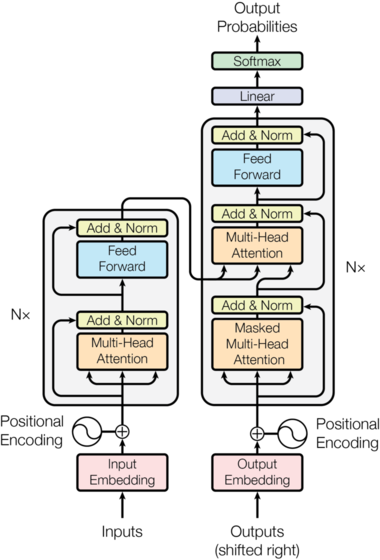
\includegraphics[width=0.4\textwidth]{resources/overview-transformer.png}
        \caption{Ilustrasi \textit{transformer} secara keseluruhan \parencite{AttentionVaswani2017}.}
        \label{fig:ilustrasi_transformer}
    \end{figure}

    Fungsi \textit{attention} dapat digambarkan sebagai memetakan kueri dan pasangan \textit{key-value} untuk suatu output, di mana kueri (Q), kunci (K), nilai (V), dan \textit{output} semuanya vektor. \textit{Output} dihitung sebagai \textit{weighted sum} dari nilai-nilai, di mana bobot yang ditetapkan untuk setiap nilai dihitung oleh fungsi kompatibilitas kueri dari kunci yang sesuai.

    Pada penelitian \parencite{AttentionVaswani2017}, tipe \textit{attention} ini disebut "\textit{Scaled Dot-Product Attention}". Input terdiri dari kueri dan kunci dimensi \(d_{k}\), dan nilai dimensi \(d_{v}\). \textit{Dot product} dari kueri dihitung dengan semua kunci, membaginya dengan \(\sqrt{d_{k}}\), dan menerapkan fungsi softmax untuk mendapatkan bobot pada nilai. Ilustrasi \textit{attention} dapat dilihat pada Gambar \ref{fig:ilustrasi_attention}.

    \begin{figure}[ht]
        \centering
        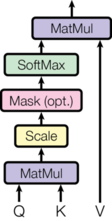
\includegraphics[width=0.2\textwidth]{resources/overview-attention.png}
        \caption{Ilustrasi \textit{attention} secara keseluruhan \parencite{AttentionVaswani2017}.}
        \label{fig:ilustrasi_attention}
    \end{figure}

    Pada prakteknya, hasil keluaran fungsi \textit{attention} pada sebuah set kueri dihitung secara besamaan, dikemas bersama menjadi matriks Q. Kunci dan nilai juga dikemas bersama menjadi matriks K dna V. Kemudian hasil keluaran dapat dihitung dengan:

    \begin{equation}
        Attention(Q,K,V) = softmax(\frac{QK^{T}}{\sqrt{d_k}})V
    \end{equation}

    Pada model MultilingualBERT dan XLM-R yang digunakan di tugas akhir ini, arsitektur Transformer menjadi kunci utama desain model. Model MultilingualBERT terdiri dari 12 blok layer Transformer, 768 \textit{hidden size}, 12 \textit{self-attention heads}, 110 ribu kosa kata, dan total 172 juta parameter. Lalu, model XLM-R Base terdiri dari terdiri dari 12 blok layer Transformer, 768 \textit{hidden size}, 12 \textit{self-attention heads}, 250 ribu kosa kata, dan total 270 juta parameter. Terakhir, model XLM-R Large terdiri dari terdiri dari 24 blok layer Transformer, 1024 \textit{hidden size}, 16 \textit{self-attention heads}, 250 ribu kosa kata, dan total 550 juta parameter.

    \subsection{Masked Language Modeling (MLM)}
    Dideskripsikan pertama kali pada penelitian \parencite{Devlin_Chang_Lee_Toutanova_2019}, \textit{Masked Language Modeling} terinspirasi dari \textit{Cloze task} \parencite{Taylor_1953}. Teknik MLM secara acak menyembunyikan beberapa kata dari input, dan model memiliki objektif untuk menebak kata asli dari kata yang disembunyikan tadi berdasarkan konteks yang ada di sekelilingnya. Tidak seperti pelatihan \textit{language model} lainnya yang berjalan dari kiri-ke-kanan, pelatihan dengan objektif MLM memungkinkan representasi dari kiri dan kanan mengambil peran. Hal ini memungkinkan pelatihan \textit{Transformer} secara dua arah. Ilustrasi dari \textit{masked language modeling} secara keseluruhan dapat dilihat pada Gambar \ref{fig:ilustrasi_mlm}.

    \begin{figure}[ht]
        \centering
        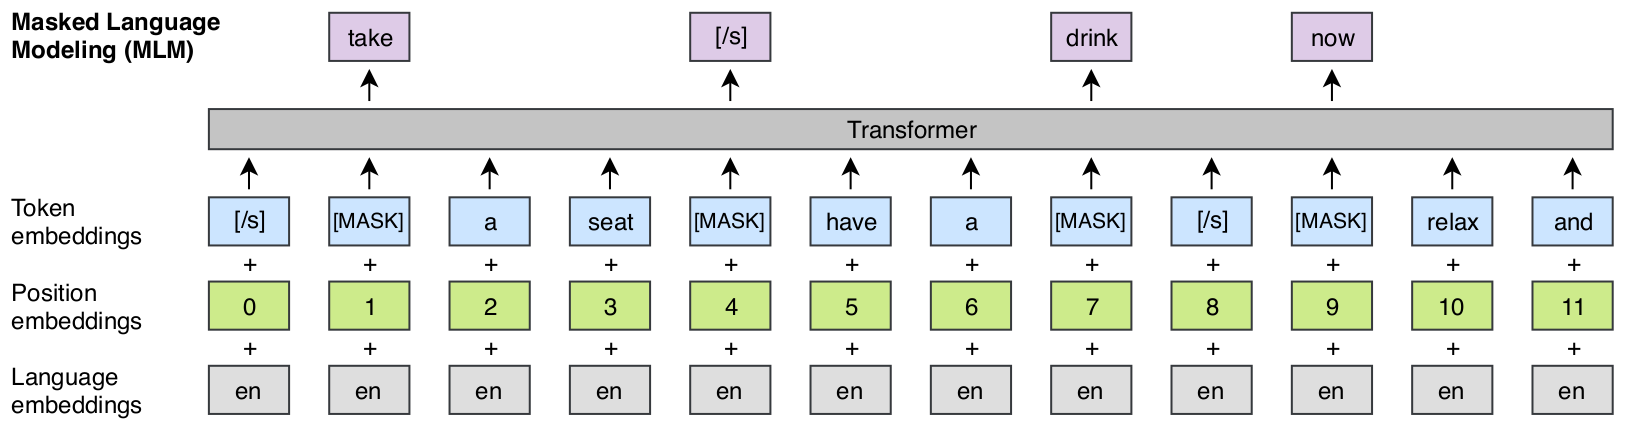
\includegraphics[width=1\textwidth]{resources/ilustrasi-mlm.png}
        \caption{Ilustrasi \textit{masked language modeling} \parencite{LampleConneau2019}.}
        \label{fig:ilustrasi_mlm}
    \end{figure}

    Sama dengan BERT, persentase dari kata yang dipilih untuk disembunyikan pada XLM adalah 15 persen. Setelah sebuah posisi dipilih secara acak, sebuah kata kemudian memiliki 80 persen kemungkinan untuk disembunyikan, 10 persen kemungkinan untuk diganti menjadi sebuah kata acak, dan 10 persen kemungkinan tidak diganti sama sekali.

    \subsection{Teknik Pretraining}
    Model BERT dan XLM merupakan perkembangan dari penelitian oleh \parencite{radford2018improving} dan \parencite{HowardRuder2018} yang meneliti \textit{language modeling} untuk melakukan \textit{pretraining Transformer encoder}. Penelitian-penelitian tersebut sukses membuktikan mangkusnya teknik ini dengan meraih kenaikan performa yang tinggi pada dataset tolak ukur GLUE \parencite{GLUE2019}.

    Teknik \textit{language model pretraining} sukses dikarenakan kemampuannya untuk memanfaatkan data-data teks yang ada dari berbagai sumber tanpa perlu melakukan pelabelan \textit{(unsupervised)}. Pada salah satu model XLM, \textit{pretraining} dilakukan pada data Wikipedia dari 100 bahasa. Melalui pembelajaran dari Wikipedia 100 bahasa ini XLM berhasil mempelajari representasi teks berbagai bahasa.

	\subsection{Teknik Fine-tuning}
	Untuk melakukan \textit{fine-tuning} model klasifikasi teks biner, sebuah \textit{dense layer} ditambahkan di atas keluaran dari \textit{language model} yang sudah di-\textit{pretrained}. Hal ini sama dengan teknik yang \parencite{LampleConneau2019} lakukan pada masalah klasifikasi antar bahasa dengan dataset XNLI \parencite{Conneau_Rinott_Lample_Williams_Bowman_Schwenk_Stoyanov_2018}. Penelitian, \parencite{Devlin_Chang_Lee_Toutanova_2019} mendefinisikan dua teknik \textit{fine-tuning} yang biasa dilakukan adalah melatih keseluruhan model atau hanya menggunakan \textit{language model} untuk mengekstraksi fitur dan kemudian melatih layer terakhir saja. Berikut penjelasan dan ilustrasi mengenai dua teknik tersebut
	\begin{enumerate}
		\item \textbf{Hanya Layer Terakhir}\\	
		Melatih	model secara keseluruhan memerlukan waktu dan sumber daya yang besar. Waktu dapat dipersingkat dengan membekukan dan tidak melatih lebih lanjut komponen \textit{multilingual language model} yang sudah mempelajari representasi teks antar bahasa. Komponen yang dilatih hanyalah \textit{dense layer} yang baru ditambahkan di atas model untuk melakukan klasifikasi. Ilustrasi dari proses ini dapat dilihat pada Gambar \ref{fig:ilustrasi_head_fine_tune}.

        Teknik \textit{fine-tuning} seperti ini memang menghasilkan performa yang lebih rendah dibanding melakukan \textit{fine-tuning} penuh seluruh arsitektur. Hal ini dikarenakan penggunaan representasi teks lintas bahasa yang murni dari hasil \textit{pretraining} sebagai fitur dan tidak dilakunannya penyempurnaan representasi ke permasalahan yang sedang diselesaikan. Tetapi walaupun begitu, efek dari penggunaan \textit{multilingual language model} dalam memanfaatkan bahasa yang lebih banyak sumber dayanya ke permasalahan bahasa Indonesia tetap dapat diobservasi.
        
        \begin{figure}[h]
            \centering
            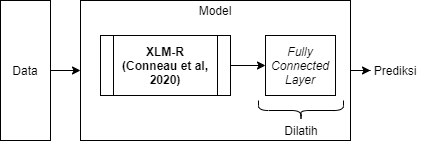
\includegraphics[width=0.75\textwidth]{resources/Head-fine-tune.png}
            \caption{ Ilustrasi \textit{fine-tuning} layer terakhir}
            \label{fig:ilustrasi_head_fine_tune}
        \end{figure}

		\item \textbf{Penuh}\\
        Pada teknik \textit{fine-tuning} full, seluruh arsitektur dilatih dengan fungsi \textit{loss} dari hasil klasifikasi. Dengan teknik ini, potensi secara keseluruhan dari \textit{pretrained multilingual language model} dapat diobservasi. Ilustrasi dari proses ini dapat dilihat pada Gambar \ref{fig:ilustrasi_full_fine_tune}.
        
        \begin{figure}[h]
            \centering
            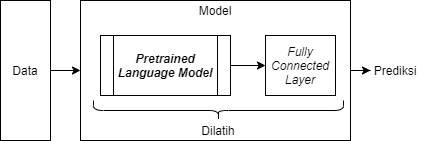
\includegraphics[width=0.75\textwidth]{resources/Full-fine-tune.png}
            \caption{ Ilustrasi \textit{fine-tuning} penuh}
            \label{fig:ilustrasi_full_fine_tune}
        \end{figure}
		
	\end{enumerate}

\section{Representasi Teks Lintas Bahasa}
    Representasi teks lintas bahasa diperlukan untuk dapat memanfaatkan bahasa Inggris dalam melatih model untuk klasifikasi teks bahasa Indonesia. Representasi teks lintas bahasa berarti merepresentasi bahasa pada ruang yang sama seperti dapat dilihat pada ilustrasi di gambar \ref{fig:ilustrasi_embedding}.

    \begin{figure}[ht]
        \centering
        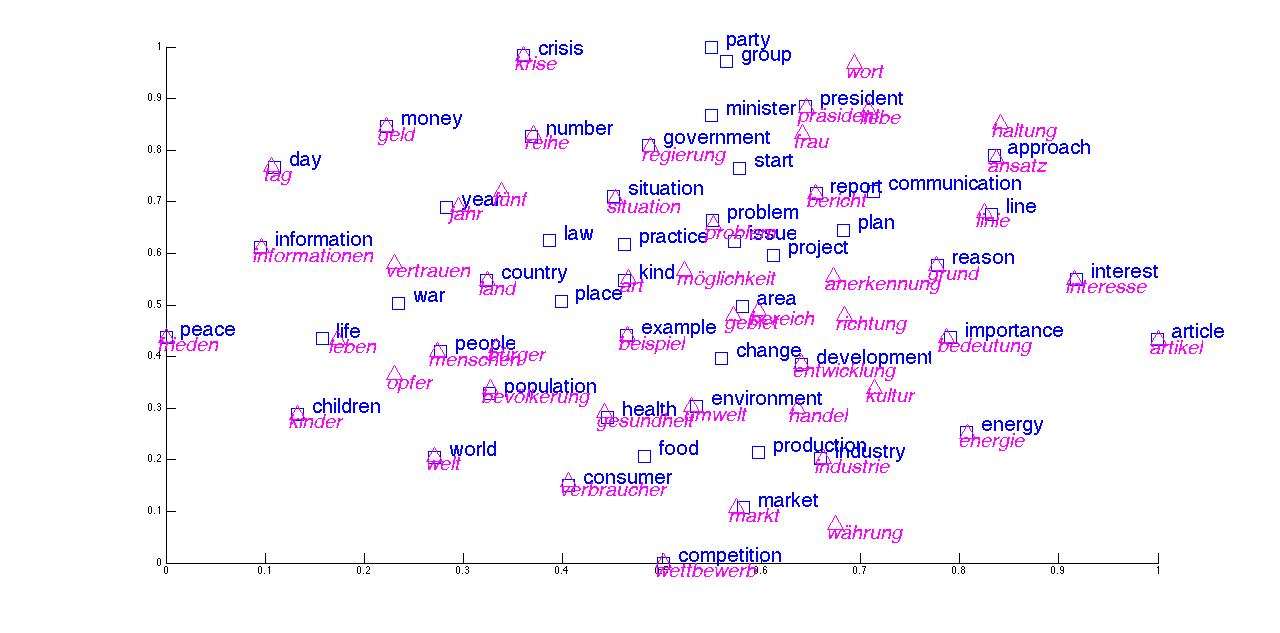
\includegraphics[width=1\textwidth]{resources/luong_et_al_2015.jpg}
        \caption{Ilustrasi ruang \textit{embedding} antara dua bahasa \parencite{Luong_Pham_Manning_2015}} 
        \label{fig:ilustrasi_embedding}
    \end{figure}

    Sebelumnya, diperlukan ahli untuk membangun kamus kata-kata dan kalimat secara manual untuk dapat membandingkan kata dari dua bahasa. Seiring dengan perkembangan teknologi, berbagai teknik berkembang untuk dapat melakukan hal ini secara otomatis. Berdasarkan \parencite{Wang_Xie_Xu_Yang_Neubig_Carbonell_2019}, secara garis besar terdapat 2 pendekatan berbeda dalam membangun ruang \textit{embedding} antar bahasa: \textit{monolingual mapping} dan \textit{joint optimization}. Subbab selanjutnya akan membahas dua hal tersebut.

    \subsection{Monolingual Mapping}

    Pada \textit{monolingual mapping},  model dilatih secara independen pada bahasa masing-masing. Kemudian mapping antara bahasa dipelajari untuk mendapatkan representasi antar bahasa. Salah satu contohnya adalah penelitian \parencite{MikolovEstimation}. Pada penelitiannya pertama-tama dipelajari representasi bahasa menggunakan model Skip-gram atau Continuous Bag-of-Words (CBOW) yang didistribusikan. Model-model ini mempelajari representasi kata menggunakan arsitektur \textit{neural network} sederhana yang bertujuan untuk memprediksi tetangga kata. Karena kesederhanaannya, model Skip-gram dan CBOW dapat dilatih pada sejumlah besar data teks. Pada implementasi paralelnya model ini dapat belajar dari miliaran kata dalam hitungan jam.

    Baru-baru ini ditunjukkan bahwa representasi kata yang didistribusikan secara mengejutkan menangkap banyak keteraturan linguistik, dan ada banyak jenis kesamaan di antara kata-kata yang dapat dinyatakan sebagai terjemahan linear \parencite{MikolovLinguistic2013}. Misalnya, operasi vektor "raja" - "pria" + "wanita" menghasilkan vektor yang dekat dengan "ratu".

    Dua model khusus untuk mempelajari representasi kata yang dapat dilatih secara efisien pada banyak data teks adalah model Skip-gram dan CBOW yang diperkenalkan di \parencite{MikolovEstimation}. Dalam model CBOW, tujuan pelatihannya adalah untuk menggabungkan representasi kata di sekitarnya untuk memprediksi kata di tengah. Sedangkan dalam model Skip-gram, tujuan pelatihan adalah untuk mempelajari representasi kata vektor yang pandai memprediksi konteksnya dalam kalimat yang sama \parencite{MikolovEstimation}. Model arsitektur dari dua metode ini ditunjukkan pada Gambar \ref{fig:ilustrasi_cbow_skip_gram}.

    \begin{figure}[ht]
        \centering
        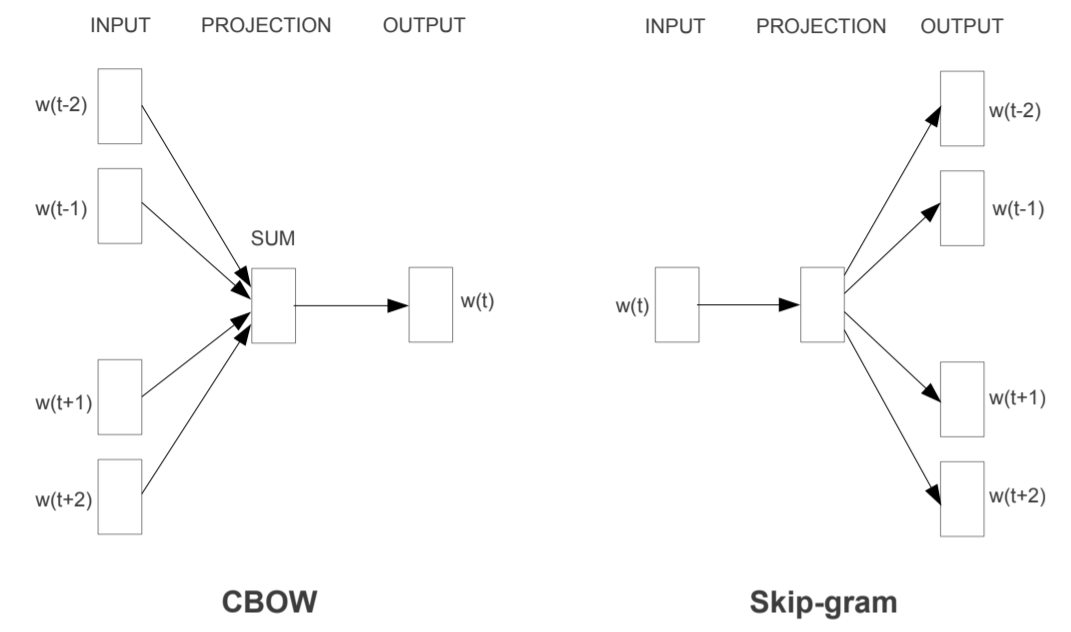
\includegraphics[width=1\textwidth]{resources/cbow-skip-gram-illustration.png}
        \caption{Ilustrasi model CBOW dan Skip-gram. \parencite{MikolovExploiting}.}
        \label{fig:ilustrasi_cbow_skip_gram}
    \end{figure}
    
    Lebih formal, diberi urutan kata pelatihan \(w1, w2, w3,. . . , wT,\) tujuan dari model Skip-gram adalah untuk memaksimalkan probabilitas log rata-rata

    \begin{equation}
        \frac{1}{T}\sum_{t=1}^{T}\begin{bmatrix}
        \sum_{j=-k}^{K}{\log p(w_{t+j}|w_{t})}
        \end{bmatrix}
        \label{eq:1}
    \end{equation}

    di mana \(k\) adalah ukuran jendela pelatihan. Iterasi penjumlahan di bagian dalam berjalan dari \({-k}\) ke \(k\) untuk menghitung probabilitas log benarnya memprediksi kata \(w_{t+j}\) jika kata di tengah \(w_{t}\). Iterasi penjumlahan di luar mencakup semua kata dalam korpus pelatihan. 

    Ketika dilatih tentang dataset besar, model Skip-gram atau CBOW ini menangkap banyak informasi semantik. Seperti yang disebutkan sebelumnya, kata-kata yang berkaitan erat memiliki representasi vektor yang serupa, misalnya, sekolah dan universitas, danau, dan sungai. Ini karena sekolah dan universitas muncul dalam konteks yang sama, sehingga selama pelatihan representasi vektor dari kata-kata ini didorong untuk menjadi dekat satu sama lain. Lebih menarik lagi, vektor menangkap hubungan antara konsep melalui operasi linier. Misalnya, \(vektor(Prancis) - vektor(Paris)\) mirip dengan \(vektor(Italia) - vektor(Roma)\).

    Pada gambar \ref{fig:ilustrasi_embedding_inggris_spanyol}, dapat dilihat visualisasi hasil pembelajaran Skip-gram atau CBOW. Gambar \ref{fig:ilustrasi_embedding_inggris_spanyol} memvisualisasikan vektor untuk angka dan hewan dalam bahasa Inggris dan Spanyol, dan dapat dengan mudah dilihat bahwa konsep-konsep ini memiliki susunan geometris yang serupa. Hal ini dikarenakan semua bahasa umum memiliki konsep yang didasarkan pada dunia nyata (seperti kucing adalah binatang yang lebih kecil dari seekor anjing), sering kali ada kesamaan kuat antara ruang vektor. Kesamaan pengaturan geometris dalam ruang vektor adalah alasan utama mengapa metode ini dapat bekerja dengan baik.

    \begin{figure}[ht]
        \centering
        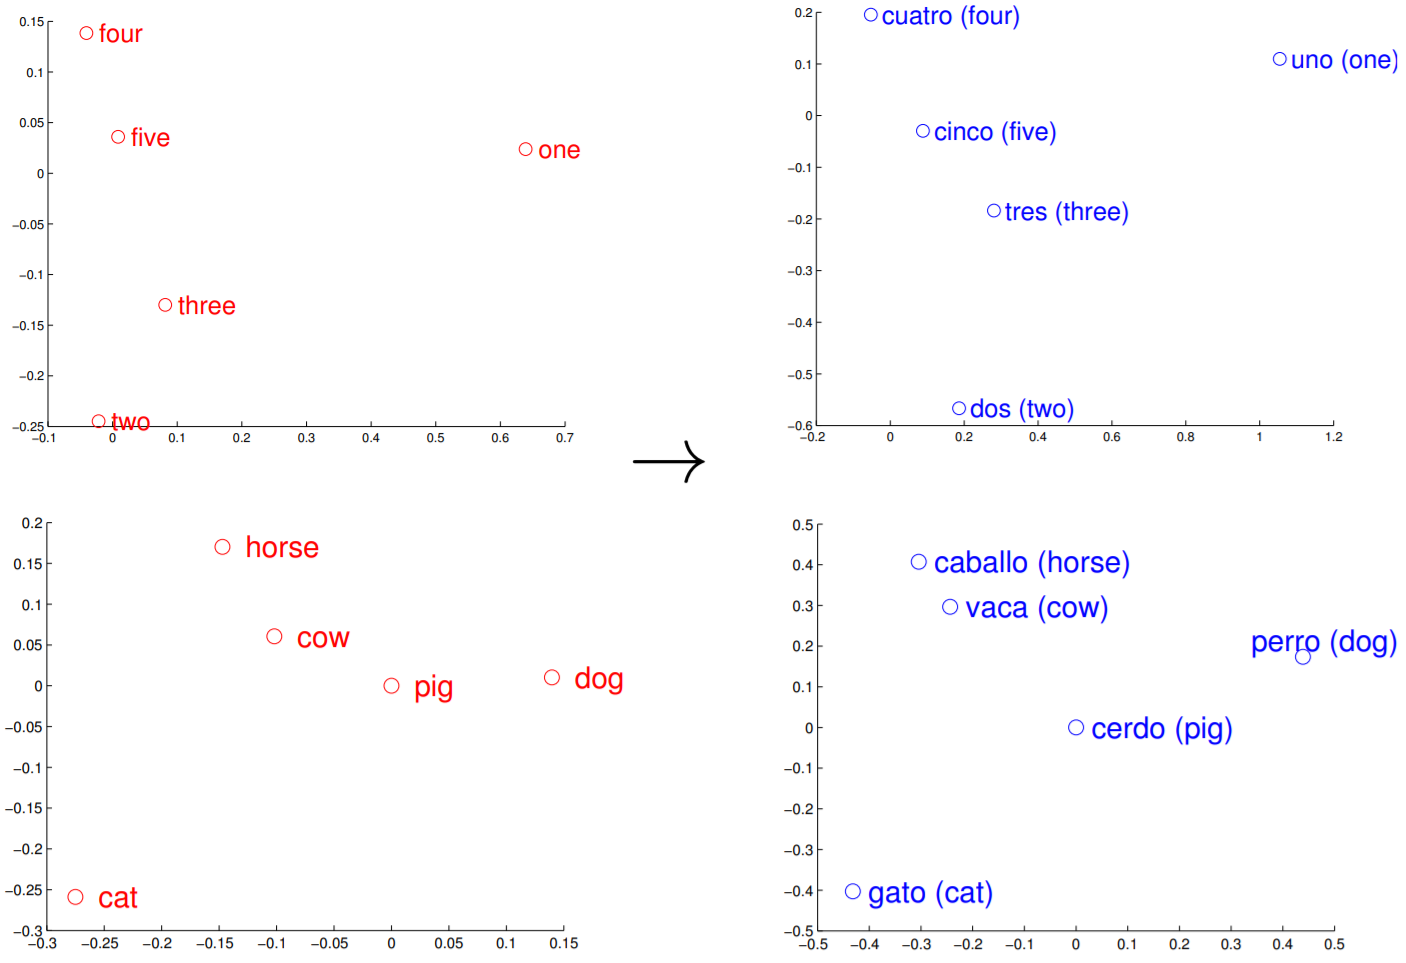
\includegraphics[width=1\textwidth]{resources/ilustration-eng-spn-word.png}
        \caption{Ilustrasi ruang \textit{embedding} antara bahasa Inggris dan Spanyol \parencite{MikolovExploiting}.}
        \label{fig:ilustrasi_embedding_inggris_spanyol}
    \end{figure}

    Dikarenakan miripnya representasi bahasa, jika translasi beberapa objek diketahui, contoh angka satu sampai lima, representasi antar bahasa dapat disesuaikan dengan rotasi, \textit{scaling}, dan translasi untuk mendapatkan translasi angka lainnya. Lebih formalnya, misalkan diberi satu set pasangan kata dan representasi vektor yang terkait \begin{math} \begin{Bmatrix} {x_{i}, z_{i}} \end{Bmatrix}_{i=1}^{n} \end{math}, di mana \(x_{i}\in\mathbb{R}^{d_{1}}\) adalah representasi terdistribusi dari kata i dalam bahasa sumber, dan \(z_{i}\in\mathbb{R}^{d_{2}}\) adalah representasi vektor dari terjemahannya. Kemudian dicari matriks transformasi \( W\) sehingga \(W x_{i}\) mendekati \(z_{i}\). Dalam praktiknya, \(W\) dapat dipelajari dengan masalah optimasi berikut

    \begin{equation}
        \min_{W}\sum_{i=1}^{n}\left \| Wx_i-z_i \right \|^2
        \label{eq:2}
    \end{equation}

    yang dapat diselesaikan dengan \textit{stochastic gradient descent} \parencite{MikolovExploiting}.

    Setiap kata baru yang diberikan dan representasi vektor kontinu \(x\) dapat dipetakan ke ruang bahasa lain dengan menghitung \(z = W x\) pada saat prediksi. Kemudian kata yang representasinya paling dekat dengan \(z\) dalam ruang bahasa target dapat ditemukan menggunakan \textit{cosine similarity} sebagai metrik jarak. Terlepas dari kesederhanaannya, metode transformasi linier ini bekerja dengan baik dalam eksperimen yang \parencite{MikolovExploiting} jalankan, lebih baik daripada teknik \textit{nearest neighbour} dan juga pengklasifikasi \textit{neural network}.

    Meski \textit{monolingual mapping} sukses mendapatkan ruang \textit{embedding} antar bahasa, teknik ini mahal dan susah diaplikasikan ke bahasa yang memiliki sumber daya rendah. Untuk dapat mengaplikasikan teknik ini diperlukan kamus kata-kata atau kalimat paralel antar bahasa, hal yang seringkali tidak tersedia pada bahasa bersumber daya rendah. Oleh karena itu, mengaplikasikan teknik ini sangat sulit pada bahasa Indonesia.
    
    \subsection{Joint Optimization}
    Pada teknik \textit{Joint Optimization}, model dilatih pada korpus dari berbagai bahasa. Model kemudian mengoptimisasi \textit{loss} dari objektif monolingual, \textit{cross-lingual}, atau kombinasi keduanya. Sebuah kemajuan terbaru dari teknik \textit{joint optimization} berhasil mengatasi permasalahan dibutuhkannya kamus paralel yang ada di teknik sebelumnya. Teknik \textit{joint optimization} yang sebelumnya memerlukan korpus paralel atau kamus bilingual (\textit{supervised}) \parencite{Xing_Wang_Liu_Lin}, kini dapat dilakukan tanpa korpus paralel atau kamus bilingual (\textit{unsupervised}) \parencite{Devlin_Chang_Lee_Toutanova_2019} \parencite{LampleConneau2019}. Penelitian \parencite{Devlin_Chang_Lee_Toutanova_2019} dan \parencite{Conneau_XLMR} melatih model pada korpus dari berbagai bahasa tanpa menggunakan objektif \textit{cross-lingual} apapun. Model yang dihasilkan telah menunjukkan kemampuan generalisasi yang baik di seluruh bahasa dan representasi agnostik bahasa di dalam keadaan tersembunyi \parencite{Pires_Schlinger_Garrette_2019}.

    Hingga saat ini, penjelasan mengenai kenapa teknik ini bekerja dengan sangat baik dalam menghasilkan representasi antar bahasa masih menjadi penelitian. Salah satu hipotesis mengenai kenapa representasi antar bahasa tersebut dapat diraih tanpa objektif antar bahasa adalah penggunaan \textit{sub-word}. Berdasarkan penelitian oleh \parencite{Sennrich_Haddow_Birch_2016}, salah satu inspirasi menggunakan \textit{sub-word} adalah fakta bahwa terjemahan beberapa kata bersifat transparan karena terjemahannya dapat diterjemahkan oleh penerjemah yang kompeten, bahkan jika itu adalah kata yang belum pernah ditemui, berdasarkan terjemahan dari \textit{sub-word} yang dikenal seperti morfemnya atau fonemnya. Kategori kata yang terjemahannya berpotensi transparan meliputi:

    \begin{enumerate}
        \item Entitas bernama (\textit{named entities}). Di antara bahasa yang menggunakan alfabet, nama seringkali dapat disalin dari sumber ke teks target. Transkripsi atau transliterasi mungkin diperlukan pada bahasa dengan huruf atau suku kata berbeda. Contoh: \\
        Barack Obama (Bahasa Inggris dan Jerman) \\
        \foreignlanguage{russian}{Барак Обама} (Bahasa Rusia) \\
        \begin{CJK}{UTF8}{min}
        バラク・オバマ (ba-ra-ku o-ba-ma) (Bahasa Jepang)
        \end{CJK}

        \item Kata-kata serumpun dan pinjaman. Kata serumpun dan kata pinjaman dengan asal yang sama dapat berbeda secara reguler antar bahasa, sehingga aturan penerjemahan tingkat karakter sudah cukup \parencite{Tiedemann2012}. Contoh:  \\
        claustrophobia (Bahasa Inggris) \\
        Klaustrophobie (Bahasa Jerman) \\
        \foreignlanguage{russian}{Клаустрофобия} (Klaustrofobiâ) (Bahasa Rusia)

        \item Kata-kata yang rumit secara morfologis. Kata-kata yang mengandung banyak morfem, misalnya yang dibentuk melalui peracikan, afiksasi, atau infleksi, dapat diterjemahkan dengan menerjemahkan morfem secara terpisah. Contoh:  \\
        solar system (Bahasa Inggris) \\
        Sonnensystem (Sonne + System) (Bahasa Jerman) \\
        Naprendszer (Nap + Rendszer) (Bahasa Hongaria)
    \end{enumerate}

    Penelitian \parencite{Sennrich_Haddow_Birch_2016} membuktikan bahwa segmentasi kata-kata langka ke dalam unit \textit{sub-word} yang sesuai sudah cukup untuk memungkinkan \textit{neural translation network} mempelajari terjemahan yang transparan, dan menggeneralisasikan pengetahuan ini untuk menerjemahkan dan menghasilkan kata-kata yang tidak ditemui sebelumnya. Pada penelitiannya, mereka menggunakan teknik \textit{Byte Pair Encoding} untuk mendapatkan tidak hanya \textit{sub-word}-nya tetapi juga kompresi dari kamus-kamus kata yang ada.

    Teknik \textit{Byte Pair Encoding} (BPE) \parencite{GageBPE1994} adalah teknik kompresi data sederhana yang secara iteratif menggantikan pasangan \textit{byte} yang paling sering muncu; secara berurutan dengan \textit{byte} tunggal yang tidak digunakan. Pada penelitiannya, \parencite{Sennrich_Haddow_Birch_2016} mengadaptasi algoritma \textit{Byte Pair Encoding} untuk segmentasi kata. Alih-alih sering menggabungkan pasangan \textit{byte}, mereka menggabungkan karakter atau urutan karakter.

    Pertama-tama, kosakata simbol diinisialisasi dengan kosakata karakter, dan mewakili setiap kata sebagai urutan karakter, ditambah simbol akhir kata khusus ‘·’, yang memungkinkan hasil terjemahan dikembalikan ke bentuk awal setelah terjemahan. Kemudian semua pasangan simbol dihitung secara iteratif dan untuk setiap pasangan yang paling sering diganti dengan simbol baru. Contoh ('A', 'B') menjadi 'AB'. Setiap operasi penggabungan menghasilkan simbol baru yang mewakili \textit{n-gram} dari karakter. Karakter yang sering muncul (atau seluruh kata) pada akhirnya digabungkan menjadi satu simbol. Ukuran kosa kata simbol akhir sama dengan ukuran kosa kata awal, ditambah jumlah operasi penggabungan --- yang merupakan satu-satunya \textit{hyperparameter} dari algoritma.

    Dapat dilihat contoh sederhana algoritma \textit{Byte Pair Encoding} pada Lampiran \ref{appendix:simple_bpe_algorithm} oleh \parencite{Sennrich_Haddow_Birch_2016}. Pada algoritma ini, operasi \textit{Byte Pair Encoding} belajar dari kamus kata {‘low’, ‘lower’, ‘newest’, ‘widest’}. Pada akhir iterasi, diperoleh representasi dari kamus kata dalam bentuk simbol-simbol yang dipelajari. Pada contoh tersebut, kata 'lowest' yang berada diluar kamus kata direpresentasikan menjadi gabungan dari simbol 'low' dan 'est'. Di sini dapat dilihat bagaimana \textit{Byte Pair Encoding} dapat membantu merepresentasikan kata yang berada diluar kamus kata. 

    Namun penelitian \parencite{K_Wang_Mayhew_Roth_2020} berhasil mematahkan hipotesis penggunaan \textit{sub-word} ini dengan melatih model menggunakan data yang sama sekali tidak memiliki \textit{sub-word} tumpang tindih. Hasil dari penelitiannya membuktikan bahwa tumpang tindih leksikal antara bahasa memainkan peran yang dapat diabaikan dalam keberhasilan lintas bahasa. Oleh karena itu, penelitian dalam menjelaskan efektifitas teknik ini masih gencar dilakukan.

\section{Multilingual Language Model}
    Bab ini menjelaskan detail dari dua \textit{multilingual language model} yang digunakan dalam tugas akhir ini: MultilingualBERT dan XLM-RoBERTa.

    \subsection{MultilingualBERT}
        MultilingualBERT adalah salah satu model yang penelitian \parencite{Devlin_Chang_Lee_Toutanova_2019} rilis. Model ini pada dasarnya memiliki arsitektur sama dengan varian BERT-Base yang terdiri dari 12 blok layer Transformer, 768 \textit{hidden size}, 12 \textit{self-attention heads}, dan total 110 juta parameter. Hanya saja model ini tidak dilatih dengan data dari BooksCorpus (800 juta kata) dan Wikipedia bahasa Inggris (2,5 miliar kata). Melainkan, model ini dilatih dengan data Wikipedia dari lebih 104 bahasa.
        
        Meski tidak didesain secara eksplisit untuk memiliki representasi antar bahasa, penelitian \parencite{Pires_Schlinger_Garrette_2019} menunjukkan bahwa MultilingualBERT memiliki kemampuan generalisasi antar bahasa yang sangat baik. Pada penelitiannya, \parencite{Pires_Schlinger_Garrette_2019} mendemonstrasikan kemampuan MultilingualBERT pada berbagai permasalahan dan menyiratkan terdapatnya informasi linguistik yang berguna antar bahasa  pada representasi di dalam MultilingualBERT

    \subsection{XLM-RoBERTa}
        XLM-RoBERTa adalah model yang dirilis dari hasil penelitian \parencite{Conneau_XLMR}. Penelitian ini mengembangkan hasil penelitian \parencite{LampleConneau2019} dengan data lebih banyak, data yang lebih beragam, dan teknik pelatihan yang lebih optimal. Model yang dirilis memiliki dua varian, XLM-R Base dan XLM-R Large. Model XLM-R Base terdiri dari terdiri dari 12 blok layer Transformer, 768 \textit{hidden size}, 12 \textit{self-attention heads}, dan total 270 juta parameter. Terakhir, model XLM-R Large terdiri dari terdiri dari 24 blok layer Transformer, 1024 \textit{hidden size}, 16 \textit{self-attention heads}, dan total 550 juta parameter. 

        Meski MultilingualBERT memiliki kemampuan generalisasi antar bahasa, masih terdapat banyak kekurangan yang menghambat kemampuan generalisasi ini maju.
        Penelitian berjudul "RoBERTa: Pendekatan Pretraining BERT yang Lebih Optimal" oleh \parencite{Liu_Ott_Goyal_Du_Joshi_Chen_Levy_Lewis_Zettlemoyer_Stoyanov_2019} menunjukkan bahwa teknik pelatihan dan beberapa pilihan desain dalam pemodelan BERT tidak optimal. Lalu dalam pembangunannya BERT juga tidak didesain dan dioptimisasi secara khusus untuk dapat generalisasi antar bahasa, hal yang \parencite{Conneau_XLMR} teliti dan perbaiki. Subbab selanjutnya membahas beberapa hal tersebut dengan lebih detail.


        \begin{table}[tb]
            \centering
            \caption{Rangkuman perbandingan objektif pelatihan \parencite{Liu_Ott_Goyal_Du_Joshi_Chen_Levy_Lewis_Zettlemoyer_Stoyanov_2019} }
            \begin{tabular}{|l|l|l|l|l|}
                \hline
                \textbf{Model} & \textbf{SQuAD 1.1/2.0} & \textbf{MNLI-m} & \textbf{SST-2} & \textbf{RACE} \\ \hline
                \multicolumn{5}{|l|}{\textit{Dengan NSP Loss:}}                                            \\ \hline
                SEGMENT-PAIR   & 90.4/78.7              & 84.0            & \textbf{92.9}  & 64.2          \\ \hline
                SENTENCE-PAIR  & 88.7/76.2              & 82.9            & 92.1           & 63.0          \\ \hline
                \multicolumn{5}{|l|}{\textit{Tanpa NSP Loss:}}                                             \\ \hline
                FULL-SENTENCES & 90.4/79.1              & \textbf{84.7}   & 92.5           & 64.8          \\ \hline
                DOC-SENTENCES  & \textbf{90.6/79.7}     & \textbf{84.7}   & 92.7           & \textbf{65.6} \\ \hline
            \end{tabular}
            \label{tab:rangkuman_roberta_1}
        \end{table}

        \subsection{Perubahan dari Desain BERT: Next Sentence Prediction dan Static Masking}
        Penelitian \parencite{Liu_Ott_Goyal_Du_Joshi_Chen_Levy_Lewis_Zettlemoyer_Stoyanov_2019} mengevaluasi kembali desain kunci pada pelatihan BERT. BERT memiliki dua objektif pelatihan, \textit{Masked Language Model (MLM)} dan \textit{Next Sentence Prediction (NSP)}. Sedangkan pada cara \textit{masking} data untuk MLM, data di-\textit{mask} secara static. Berarti selama pelatihan, teks yang di-\textit{mask} hanya itu saja dan tidak berubah. Dua Desain kunci ini adalah beberapa hal yang dievaluasi oleh \parencite{Liu_Ott_Goyal_Du_Joshi_Chen_Levy_Lewis_Zettlemoyer_Stoyanov_2019}.

        Pada objektif pelatihan, \parencite{Liu_Ott_Goyal_Du_Joshi_Chen_Levy_Lewis_Zettlemoyer_Stoyanov_2019} membandingkan dengan cermat penggunaan objektif NSP pada berbagai tipe cara memasukkan data kedalam pelatihan model. Hasil perbandingan menunjukkan bahwa penghilangan objektif NSP berefek bagus atau sama saja pada performa model. Rangkuman hasil perbandingan dapat dilihat pada Tabel \ref{tab:rangkuman_roberta_1}.

        \begin{table}[b]
            \centering
            \caption{Rangkuman perbandingan teknik \textit{masking} \parencite{Liu_Ott_Goyal_Du_Joshi_Chen_Levy_Lewis_Zettlemoyer_Stoyanov_2019} }
            \begin{tabular}{lccc}
                \hline
                \textbf{Masking} & \textbf{SQuAD 1.1/2.0} & \textbf{MNLI-m} & \textbf{SST-2} \\ \hline
                \textit{static}  & 78.3                   & \textbf{84.3}   & 92.5           \\
                \textit{dynamic} & \textbf{78.7}          & 84.0            & \textbf{92.9}  \\ \hline
            \end{tabular}
            \label{tab:rangkuman_roberta_2}
        \end{table}

        Pada cara \textit{masking} data untuk MLM, \parencite{Liu_Ott_Goyal_Du_Joshi_Chen_Levy_Lewis_Zettlemoyer_Stoyanov_2019} membandingkan dengan cermat efek dari melakukan \textit{masking} hanya sekali pada seluruh data pelatihan (\textit{static}) dengan melakukan \textit{masking} tiap kali data diproses oleh model (\textit{dynamic}). Hasil perbandingan menunjukkan bahwa teknik \textit{masking} \textit{dynamic} dalam sebagian besar kasus lebih baik dibandingkan \textit{static}. Dengan begitu, menimbang lebih efisiennya teknik \textit{dynamic}, ditetapkan bahwa teknik \textit{dynamic} lebih bagus. Rangkuman hasil perbandingan dapat dilihat pada Tabel \ref{tab:rangkuman_roberta_2}.

        \subsection{Penambahan dan Penyeimbangan Data}
        XLM-R Dilatih dengan data yang lebih banyak dan lebih beragam. Dapat dilihat pada \ref{fig:data_xlm_r} Jumlah data dalam GiB (skala log) untuk 88 bahasa yang muncul di Wiki-100 corpus yang digunakan untuk mBERT, dan CC-100 yang digunakan untuk XLM-R. CC-100 meningkatkan jumlah data secara signifikan, khususnya untuk bahasa sumber daya rendah.

        \begin{figure}[ht]
            \centering
            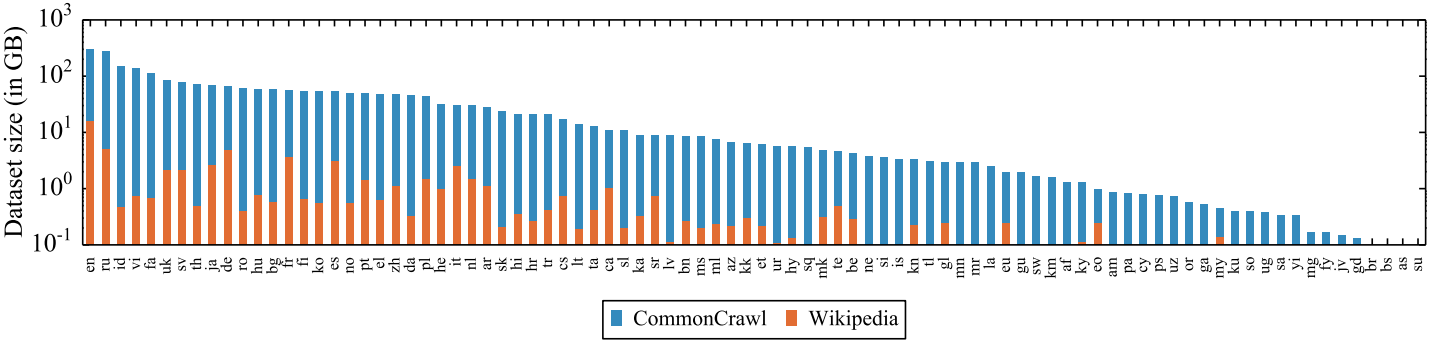
\includegraphics[width=1\textwidth]{resources/data_xlm_r.png}
            \caption{Perbedaan data mBERT (Wikipedia) dengan XLM-R (CC) \parencite{Conneau_XLMR}}
            \label{fig:data_xlm_r}
        \end{figure}

        Penambahan data dan penyeimbangan persentasenya ini terbukti meningkatkan performa model dalam berbagai permasalahan klasifikasi, terutama di bahasa yang sebelumnya memiliki lebih sedikit data. Hal ini dibuktikan dari performa model pada tolak ukur XNLI. Model XLM-R Large berhasil mendapatkan performa terbaik dalam seluruh bahasa tolak ukur XNLI. Bahkan meningkat jauh dari penelitian \parencite{LampleConneau2019} sebelumnya. Peningkatan paling nampak pada bahasa yang memiliki sumber daya sedikit.

\section{Metrik Evaluasi}
Metrik yang digunakan mengacu pada penelitian terkait sebelumnya agar dapat dibandingkan. Untuk mengevaluasi performa klasifikasi ujaran kebencian, digunakan akurasi. Sedangkan untuk mengevaluasi performa dari analisis sentimen yang dilakukan pada bahasa Indonesia, digunakan \textit{f1-score}. \textit{f1-score} adalah rata-rata harmonis antara \textit{precision} dan \textit{recall}. 

Precision merupakan rasio prediksi benar positif dibandingkan dengan keseluruhan hasil yang diprediksi positif. Precision menjawab pertanyaan " Berapa persen teks yang benar memiliki sentimen positif dari keseluruhan mahasiswa yang diprediksi memiliki sentimen positif". Definisi dari \textit{precision} secara matematis dapat dilihat pada persamaan \ref{eq:precision}.
\begin{equation}
    precision=\frac{True Positive}{True Positive + False Positive}
    \label{eq:precision}
\end{equation}

Recall merupakan rasio prediksi benar positif dibandingkan dengan keseluruhan data yang benar positif. Recall menjawab pertanyaan "Berapa persen teks yang diprediksi memiliki sentimen positif dibandingkan keseluruhan teks yang sebenarnya memiliki sentimen positif". Definisi dari \textit{recall} secara matematis dapat dilihat pada persamaan \ref{eq:recall}.
\begin{equation}
    recall=\frac{True Positive}{True Positive + False Negative}
    \label{eq:recall}
\end{equation}

Sehingga terakhir, definisi dari \textit{f1-score} secara matematis dapat dilihat pada persamaan \ref{eq:f1-score}. 
\begin{equation}
    f1-score=2.\: \frac{precision\: .\: recall}{precision+recall}
    \label{eq:f1-score}
\end{equation}

Dengan pengelompokkan prediksi sesuai dengan \textit{confusion matrix} pada tabel \ref{tab:confusion_matrix}.
\begin{table}[ht]
    \centering
    \begin{tabular}{@{}cc|cc@{}}
    \multicolumn{1}{c}{} &\multicolumn{1}{c}{} &\multicolumn{2}{c}{Prediksi} \\ 
    \multicolumn{1}{c}{} & 
    \multicolumn{1}{c|}{} & 
    \multicolumn{1}{c}{\textit{True}} & 
    \multicolumn{1}{c}{\textit{False}} \\ 
    \cline{2-4}
    \multirow[c]{2}{*}{\rotatebox[origin=tr]{90}{Label}}
    & \textit{True}  & \textit{True Positive} & \textit{False Negative}   \\[1.5ex]
    & \textit{False}  & \textit{False Positive}   & \textit{True Negative} \\ 
    \cline{2-4}
    \end{tabular}
    \caption{Tabel \textit{Confusion matrix}.}
    \label{tab:confusion_matrix}
\end{table}

\section{Penelitian Terkait}
Sebelumnya belum terdapat penelitian, dalam bahasa apapun, yang memanfaatkan dan menganalisa pengaruh penggunaan \textit{multilingual language model} untuk menambah data pelatihan dalam permasalahan analisis sentimen dan klasifikasi ujaran kebencian. Tetapi dalam permasalahan analisis sentimen dan klasifikasi ujaran kebencian bahasa Indonesia, telah banyak penelitian terkait. Penelitian tersebut adalah \parencite{FarhanKhodra2017}, \parencite{CrisdayantiPurwarianti2019}, dan \parencite{Ibrohim_Budi_2019}. Untuk pemanfaatan \textit{multilingual language model} dalam klasifikasi teks diluar bahasa Indonesia, sudah terdapat penelitian oleh \parencite{LampleConneau2019} dalam permasalahan klasifikasi apakah sebuah pasangan teks berkaitan, kontradiksi, atau netral. 

\textbf{Pada penelitian \parencite{FarhanKhodra2017}} yang berjudul “\textit{Sentiment-specific word embedding for Indonesian sentiment analysis}”, berbagai bentuk representasi teks dibandingkan dan dievaluasi menggunakan dataset ulasan TripAdvisor. Hasil dari penelitian ini dapat dilihat pada Tabel \ref{tab:FarhanKhodra2017}.
\begin{table}[!h]
    \centering
    \caption{Sebagian hasil eksperimen penelitian \parencite{FarhanKhodra2017}.}
    \begin{tabular}{|l|l|l|}
    \hline
    \multicolumn{1}{|c|}{\multirow{2}{*}{\textbf{Word Embedding}}} & \multicolumn{2}{c|}{\textbf{Hasil Evaluasi}}                                                    \\ \cline{2-3} 
    \multicolumn{1}{|c|}{}                                         & \multicolumn{1}{c|}{\textbf{10-fold cross validation}} & \multicolumn{1}{c|}{\textbf{Data Uji}} \\ \hline
    Bag of words                                                   & 0.8345                                                 & 0.8232                                 \\ \hline
    TF-IDF                                                         & \textbf{0.8492}                                        & \textbf{0.8521}                        \\ \hline
    % Word2Vec                                                       & 0.7204                                                 & 0.7219                                 \\ \hline
    % SSWE dari W2V                                                  & 0.7311                                                 & 0.7224                                 \\ \hline
    SSWE                                                           & 0.7623                                                 & 0.7687                                 \\ \hline
    \end{tabular}
    \label{tab:FarhanKhodra2017}
\end{table} 

\textbf{Pada penelitian \parencite{CrisdayantiPurwarianti2019}} yang berjudul “\textit{Improving Bi-LSTM Performance for Indonesian Sentiment Analysis Using Paragraph Vector}”, dilakukan perbandingan berbagai representasi dokumen dan topologi \textit{neural network}. Hasil terbaik didapatkan oleh model yang dilatih pada representasi kata dengan TF-IDF dan representasi paragraf dengan Doc2vec. Model Bi-LSTM yang dilatih berhasil mendapatkan F1-Score sebesar 0.9369 pada data sentimen dari berbagai media sosial (Twitter, Zomato, TripAdvisor, Facebook, Instagram, Qraved). Hasil dari penelitian ini dapat dilihat pada Tabel \ref{tab:CrisdayantiPurwarianti2019}.

\begin{table}[!h]
    \centering
    \caption{Hasil penelitian \parencite{CrisdayantiPurwarianti2019}.}
    \begin{tabular}{|l|l|l|l|}
    \hline
    \multicolumn{1}{|c|}{\textbf{Model}} & \multicolumn{1}{c|}{\textbf{Precision}} & \multicolumn{1}{c|}{\textbf{Recall}} & \textbf{F1-Score} \\ \hline
    SVM (TF-IDF)                         & 0.7977                                  & 0.8878                               & 0.8658            \\ \hline
    Bi-LSTM (WE)                         & 0.9166                                  & 0.9126                               & 0.9125            \\ \hline
    Bi-LSTM (PV+WE)                      & \textbf{0.9384}                         & \textbf{0.9369}                      & \textbf{0.9369}   \\ \hline
    \end{tabular}
    \label{tab:CrisdayantiPurwarianti2019}
\end{table}

\textbf{Pada penelitian \parencite{Ibrohim_Budi_2019}} yang berjudul "\textit{Multi-label Hate Speech and Abusive Language Detection in Indonesian Twitter}", dilakukan klasifikasi multi-label ujaran kebencian \& kasar. Dataset ujaran kebencian \& kasar tersebut merupakan \textit{tweet} dari sosial media Twitter\footnote{\url{https://www.twitter.com/}} yang dianotasi oleh 30 anotator dengan berbagai etnis, agama, dan pekerjaan. 

Terdapat dua skenario eksperimen yang dicoba. Pada skenario pertama, klasifikasi dilakukan hingga ke target, kategori, dan levelnya. Pada skenario kedua, klasifikasi hanya dilakukan sampai menentukan kategori teks ujaran kebencian atau kasar saja. Skenario kedua ini lah yang paling dekat dengan tugas akhir ini. Dalam eksperimennya, metrik yang diperhatikan adalah rata-rata dari akurasi prediksi terhadap masing-masing label. Hasil skenario kedua dapat dilihat pada Tabel \ref{tab:Ibrohim_Budi_2019_2}

\begin{table}[hbt]
    \centering
    \caption{Hasil klasifikasi ujaran kebencian \parencite{Ibrohim_Budi_2019}.}
    \begin{tabular}{|l|l|l|}
    \hline
    \textbf{Tipe Fitur} & \textbf{Fitur Terbaik} & \textbf{Rata-rata Akurasi (\%)} \\ \hline
    word n-gram              & word unigram                                    & 73.53                          \\ \hline
    character n-gram         & character quadgrams                             & 72.44                          \\ \hline
    ortography               & exclamation mark                                & 45.27                          \\ \hline
    lexicon                  & positive sentiment + abusive lexicon            & 52.10                          \\ \hline
    \end{tabular}
    \label{tab:Ibrohim_Budi_2019_2}
\end{table}

\begin{table}[!h]
    \centering
    \caption{Hasil pada uji akurasi di dataset XNLI \parencite{LampleConneau2019}.}
    \begin{tabular}{|l|l|l|l|l|}
    \hline
    \multicolumn{1}{|c|}{\textbf{Evaluasi \textit{Sentence Encoder} Lintas Bahasa}} & \multicolumn{1}{c|}{\textbf{en}} & \multicolumn{1}{c|}{\textbf{fr}} & \textbf{es}   & \textbf{de}   \\ \hline
    \parencite{LamplePhrase2018}                            & 73.7                             & 67.7                             & 68.7          & 67.7          \\ \hline
    \parencite{Devlin_Chang_Lee_Toutanova_2019}         & 81.4                             & -                                & 74.3          & 70.5          \\ \hline
    \parencite{Artetxe_Schwenk_2019}                      & 73.9                             & 71.9                             & 72.9          & 72.6          \\ \hline
    \parencite{LampleConneau2019}                           & \textbf{83.2}                    & \textbf{76.5}                    & \textbf{76.3} & \textbf{74.2} \\ \hline
    \end{tabular}
    \label{tab:LampleConneau2019}
\end{table}

\textbf{Pada penelitian \parencite{LampleConneau2019}} yang berjudul “\textit{Cross-lingual Language Model Pretraining}”, model berarsitektur \textit{transformer} dilatih dengan MLM dan \textit{shared sub-word vocabulary} pada data Wikipedia. Kemudian keluaran dari \textit{layer} terakhir model ini menjadi masukan ke \textit{layer} linier terakhir. Model mereka berhasil memecahkan beberapa state-of-the-art pada  dataset tolak ukur klasifikasi pembelajaran lintas bahasa XNLI \parencite{Conneau_Rinott_Lample_Williams_Bowman_Schwenk_Stoyanov_2018}. Hasil dari penelitian ini dapat dilihat pada Tabel \ref{tab:LampleConneau2019}. Hasil yang ditampilkan hanya 4 dari 15 bahasa dan hanya hasil XLM dengan pendekatan \textit{unsupervised}.




    \chapter{Analisis dan Rancangan Klasifikasi Teks Berbahasa Indonesia Menggunakan \textit{Multilingual Language Model}}

Bab ini berisi analisis dan rancangan berkaitan dengan studi literatur pada bab sebelumnya. Oleh karena itu, bab ini terdiri dari analisis permasalahan dan rancangan solusi.

\section{Analisis Permasalahan}
	Subbab ini berisi analisis dari dua permasalahan klasifikasi teks yang akan diselesaikan, yaitu analisis sentimen dan klasifikasi ujaran kebencian.

	\subsection{Analisis Permasalahan Analisis Sentimen}
	Pada penelitian ini, digunakan dua buah dataset. Dataset pertama, dirujuk sebagai dataset A, adalah dataset yang sama dengan penelitian \parencite{FarhanKhodra2017}. Dataset tersebut merupakan ulasan-ulasan dari situs TripAdvisor yang kemudian dilabeli positif untuk nilai 3-5 dan negatif untuk nilai 1-2. Detail dari dataset ini dapat dilihat pata \ref{tab:detail_sentiment_a}

	\begin{table}[ht]
	    \centering
	    \caption{Rincian dataset \parencite{FarhanKhodra2017}}
	    \begin{tabular}{@{}cc|cc@{}}
			\multicolumn{1}{c}{} &\multicolumn{1}{c}{} &\multicolumn{2}{c}{Partisi} \\ 
			\multicolumn{1}{c}{} & 
			\multicolumn{1}{c|}{} & 
			\multicolumn{1}{c}{\textit{Train}} & 
			\multicolumn{1}{c}{\textit{Test}} \\ 
			\cline{2-4}
			\multirow[c]{2}{*}{\rotatebox[origin=tr]{90}{Label}}
			& Positif  & 6.281 & 1.125   \\[1.5ex]
			& Negatif  & 6.108 & 1.304   \\ 
			\cline{2-4}
	    \end{tabular}
	    \label{tab:detail_sentiment_a}
	\end{table}
	
	Dataset kedua, dirujuk sebagai dataset B,  dan dataset dari Prosa.ai \parencite{CrisdayantiPurwarianti2019}. Dataset tersebut berupa kumpulan teks Twitter, Zomato, Facebook, Instagram, Qraved yang sudah dianotasi oleh annotator profesional. Setiap ulasan, yang terdiri dari satu sampai tiga kalimat, dapat memiliki frasa sentimen di awal, di tengah, dan di akhir dokumen. Detail dari dataset ini dapat dilihat pata \ref{tab:detail_sentiment_b}.

	\begin{table}[ht]
	    \centering
	    \caption{Rincian dataset \parencite{CrisdayantiPurwarianti2019}}
	    \begin{tabular}{@{}cc|cc@{}}
			\multicolumn{1}{c}{} &\multicolumn{1}{c}{} &\multicolumn{2}{c}{Partisi} \\ 
			\multicolumn{1}{c}{} & 
			\multicolumn{1}{c|}{} & 
			\multicolumn{1}{c}{\textit{Train}} & 
			\multicolumn{1}{c}{\textit{Test}} \\ 
			\cline{2-4}
			\multirow[c]{2}{*}{\rotatebox[origin=tr]{90}{Label}}
			& Positif  & 7.151 & 208   \\[1.5ex]
			& Negatif  & 3.830 &204   \\ 
			\cline{2-4}
	    \end{tabular}
	    \label{tab:detail_sentiment_b}
	\end{table}

	Berikut contoh ulasan yang berlabel negatif:

	“Kemaren sengaja coba makan di marugame udon karena istri suka banget sama udon. jadi pesan lah yang kuah kaldu ayam, dan anak saya minta gorengan kroket. saya kira kuahnya langsung dari pancinya harusnya panas, tapi ternyata cuman hangat, yah kecewa juga sih, gorengannya juga sama udah dingin” 

	Dapat dilihat dari paragraf di atas, kalimat awal pada paragraf tersebut tidak mengandung sentimen apapun. Frasa sentimen baru ditemui di akhir paragraf. Berikut contoh ulasan yang berlabel positif.

	“berlokasi di pusat jakarta.. sangat mudah mengakses ke berbagai tempat strategis dan keramaian. hotel sangat bersih, pelayanan ramah dan makanan sesuai lidah indonesia atau western. sangat direkomendasikan.”

	Dapat dilihat dari paragraf di atas, frasa sentimen positif sudah langsung diutarakan pada awal paragraf. Tetapi tidak semua ulasan memiliki satu sentimen saja. Berikut ini adalah salah satu contoh ulasan pada dataset yang mengandung frasa sentimen negatif dan positif disaat bersamaan. 

	“Kelihatan dari luar memang menarik tempatnya. Suasananya juga cozy. Saat makan siang juga ramai pengunjung. AC tidak berasa, jadi lumayan panas di dalam. Memesan nasi dengan irisan slice pork belly, nasinya tanpa bumbu apa- apa jadi kering banget, irisan pork belly nya dominan lemak dan minyak. Kita dapat 6 slice, tapi sesudah makan slice ke 3, rasanya tidak sanggup lagi karena merasa eneg dengan lemak pork belly nya.”

	Dapat dilihat dari paragraf di atas, tiga kalimat pertama menunjukkan opini positif sedangkan 3 kalimat terakhir menunjukkan opini negatif. Tetapi berdasarkan analisis keseluruhan, dapat dilihat bahwa ulasan tersebut bersentimen negatif.

	Penelitian terkait oleh \parencite{FarhanKhodra2017} dan \parencite{CrisdayantiPurwarianti2019} sudah mengekplorasi berbagai jenis representasi dokumen dan topologi untuk menyelesaikan analisis sentimen level dokumen pada data tersebut. Meski sudah mendapatkan hasil, penelitian terkait sebelumnya belum mengeksplorasi penggunaan \textit{language model} dalam bentuk apapun, terlebih lagi penggunaan \textit{transfer learning} lintas bahasa.

	Perkembangan dalam bidang teknik pemrosesan teks dewasa ini telah memunculkan berbagai jenis \textit{language model} dan teknik pembangunannya. Salah satunya adalah \textit{language model} lintas bahasa bernama XLM oleh \parencite{LampleConneau2019} yang dibangun tanpa menggunakan korpus paralel atau kamus kata antar bahasa. Hal ini memungkinkan penggunaan representasi antar bahasanya untuk melatih model analisis sentimen bahasa Indonesia dengan dataset bahasa lainnya.

	\subsection{Analisis Permasalahan Klasifikasi Teks Ujaran Kebencian \& Kasar}

	Pada penelitian ini, digunakan dataset yang sama dengan dataset \parencite{Ibrohim_Budi_2019}. Dataset tersebut merupakan \textit{tweet} dari sosial media Twitter\footnote{\url{https://www.twitter.com/}} yang dianotasi oleh 30 anotator dengan berbagai etnis, agama, dan pekerjaan. Kemudian, sesuai dengan diskusi yang \parencite{Diksusi_Bareskrim} lakukan bersama Direktorat Tindak Pidana Siber Badan Reserse Kriminal Kepolisian Negara Republik Indonesia, setiap teks tidak hanya dianotasi sebagai ujaran kebencian atau tidak, tetapi juga sampai pada target, kategori, dan levelnya. 

	Setiap teks ujaran kebencian ditujukan pada target tertentu. Secara umum, ujaran kebencian dapat ditujukan kepada individu atau grup. Kelompok yang menjadi sasaran ujaran kebencian dapat berupa asosiasi, komunitas, dan perkumpulan yang berkaitan dengan berbagaihal termasuk agama, ras, hobi, partai politik, dan lain-lain.

	Ujaran kebencian yang ditujukan baik kepada individu maupun grup kemudian dapat dilabeli berdasarkan kategori dan levelnya. Berdasarkan kategori, ujaran kebencian dapat dikategorikan sebagai berikut:
	\begin{enumerate}
		\item Agama
		\item Ras / etnis
		\item Cacat / fisik
		\item Jenis kelamin atau orientasi seksual
		\item Cercaan / fitnah lainnya
	\end{enumerate}

	Berdasarkan level, ujaran kebencian dapat dikategorikan sebagai berikut:
	\begin{enumerate}
		\item \textbf{Ujaran kebencian lemah.} Pada ujaran kebencian lemah, ujaran kebencian dengan kategori cercaan atau fitnah ditargetkan ke individu tanpa ada hasutan / provokasi untuk membuat konflik terbuka.
		\item \textbf{Ujaran kebencian sedang.} Pada ujaran kebencian sedang, ujaran kebencian dengan kategori agama, ras, stereotip ditargetkan ke grup tanpa ada hasutan / provokasi untuk membuat konflik terbuka.
		\item \textbf{Ujaran kebencian kuat.} Pada ujaran kebencian kuat, ujaran kebencian dengan kategori agama, ras, stereotip ditargetkan ke grup bersama dengan hasutan / provokasi untuk membuat konflik terbuka.
	\end{enumerate}

	Berikut beberapa contoh ujaran kebencian pada dataset yang digunakan:
	
	\begin{enumerate}
		\item \textbf{Ujaran kebencian lemah dengan kategori fisik:} \\ 
		"perempuan kaya lo mending mati aja deh, jelek aja, gausa sok jadi make up artist!"

		\item \textbf{Ujaran kebencian kuat dengan kategori jenis kelamin atau orientasi seksual:} \\
		"USER Eh dungu, ngapain lu masih mensen2 gue, katanya mau muter alun gue. Lu itu cuma bisa forward berita tanpa analisa. Kelompok MAHO mana ada yg cerdas wk wk wk"

		\item \textbf{Ujaran kebencian kuat dengan kategori ras:} \\ 
		"ARTINYA APA ? Pribumi sadari \& lihat siapa mereka ? KECUALI KALIAN sama-sama CINA KOMUNIS / MISIONARIS abaikan tweet ini usir cina Indonesia"
	\end{enumerate}

	Dalam tugas akhir ini, analisis permasalahan dilakukan tidak sampai ke kategori, target, atau levelnya. Permasalahan ini disederhakan menjadi klasifikasi biner di mana teks diklasifikasi menjadi antara ujaran kebencian \& kasar atau tidak saja. Hal ini dilakukan berhubungan dengan ketersediaan data bahasa asing yang dibicarakan pada subbab selanjutnya. Pada penelitian sebelumnya, model evaluasi digunakan dengan 10 K-Fold pada data. Pada penelitian ini, data dipartisi menjadi train dan test dengan persentase 80:20. Detail dari dataset ini dapat dilihat pata \ref{tab:detail_data_hs}.

	\begin{table}[ht]
	    \centering
	    \caption{Rincian dataset \parencite{Ibrohim_Budi_2019}}
	    \begin{tabular}{@{}cc|cc@{}}
			\multicolumn{1}{c}{} &\multicolumn{1}{c}{} &\multicolumn{2}{c}{Partisi} \\ 
			\multicolumn{1}{c}{} & 
			\multicolumn{1}{c|}{} & 
			\multicolumn{1}{c}{\textit{Train}} & 
			\multicolumn{1}{c}{\textit{Test}} \\ 
			\cline{2-4}
			\multirow[c]{2}{*}{\rotatebox[origin=tr]{90}{Label}}
			& Hate-speech  & 6.578 & 731   \\[1.5ex]
			& Normal  & 5.274 & 1.586   \\ 
			\cline{2-4}
	    \end{tabular}
	    \label{tab:detail_data_hs}
	\end{table}

	Penelitian terkait oleh \parencite{Ibrohim_Budi_2019} mengeksplorasi berbagai jenis algoritma dan fitur terbaik yang dapat digunakan untuk melakukan klasifikasi pada data tersebut. Meski sudah mendapatkan hasil, penelitian terkait sebelumnya belum mengeksplorasi penggunaan \textit{language model} dalam bentuk apapun, terlebih lagi penggunaan \textit{language model} lintas bahasa.


\section{Rancangan Solusi}
	Berdasarkan analisis permasalahan yang dijabarkan pada bab sebelumnya, \textit{language model} antar bahasa seperti XLM atau mBERT dapat digunakan untuk memperkaya analisis sentimen dan klasifikasi ujaran kebencian bahasa Indonesia. Diantara berbagai bahasa yang sudah dilatih pada \textit{language model} XLM dan mBERT adalah bahasa Indonesia dan bahasa Inggris. Subbab selanjutnya membahas pemilihan dataset bahasa Inggris yang digunakan dan rancangan eksperimen untuk membuktikan tujuan dari tugas akhir ini.

	\subsection{Dataset Bahasa Inggris Analisis Sentimen}
	Dataset bahasa Inggris yang digunakan adalah dataset ulasan pada website \textit{Yelp}\footnote{\url{https://www.yelp.com/dataset}}. Dataset dipilih dikarenakan jumlahnya dan kesesuaian domainnya dengan dataset TripAdvisor. Dataset polaritas Yelp reviews  dibangun dengan mengubah semua rating bintang 1 dan 2 menjadi negatif, dan rating bintang 3 dan 4 menjadi positif. Rincian dari dataset dapat dilihat pada tabel \ref{tab:detail_yelp_review}.

	\begin{table}[ht]
	    \centering
	    \caption{Rincian banyak data pada tiap partisi dan label di dataset \textit{Yelp review}}
	    \begin{tabular}{@{}cc|cc@{}}
			\multicolumn{1}{c}{} &\multicolumn{1}{c}{} &\multicolumn{2}{c}{Partisi} \\ 
			\multicolumn{1}{c}{} & 
			\multicolumn{1}{c|}{} & 
			\multicolumn{1}{c}{\textit{Train}} & 
			\multicolumn{1}{c}{\textit{Test}} \\ 
			\cline{2-4}
			\multirow[c]{2}{*}{\rotatebox[origin=tr]{90}{Label}}
			& Positif  & 280.000 & 19.000   \\[1.5ex]
			& Negatif  & 280.000 & 19.000   \\ 
			\cline{2-4}
	    \end{tabular}
	    \label{tab:detail_yelp_review}
	\end{table}

	Sesuainya domain antara dataset sumber dan target sangat penting dikarenakan perbedaan domain dapat menurunkan performa klasifikasi \parencite{Lai_Oguz_Yang_Stoyanov_2019}. Hal ini dikarenakan sentimen tidak diutarakan dengan cara yang sama pada domain yang berbeda. Ulasan pada domain produk di toko \textit{e-commerce} berbeda dengan ulasan pada domain restoran. Pada domain produk di toko \textit{e-commerce}, ulasan berkutat pada aspek seperti kecepatan pengiriman barang, keselamatan barang, dan kualitas dari barang yang dibeli. Sedangkan ulasan pada domain restoran berkutat pada keramahan pelayanan, suasana restoran, dan kualitas makanan.
	
	\subsection{Dataset Bahasa Inggris Klasifikasi Ujaran Kebencian \& Kasar}
	Dataset bahasa Inggris yang digunakan adalah dataset ujaran kebencian \& kasar oleh inkubator teknologi milik Google, Jigsaw\footnote{\url{https://www.kaggle.com/c/jigsaw-unintended-bias-in-toxicity-classification/data}}. Data ini berisi 1.902.194 (152.111 \textit{toxic} \& 1.750.083 normal)teks percakapan daring yang dianotasi oleh puluhan hingga ribuan annotator per teks. 

	Label utama yang menjadi fokus dataset ini adalah \textit{toxic} atau tidaknya sebuah teks. Jigsaw mendefinisikan komentar yang \textit{toxic} sebagai komentar kasar, tidak sopan, atau tidak masuk akal yang agaknya membuat Anda meninggalkan diskusi atau menyerah untuk berbagi perspektif Anda. Dapat dilihat, hal ini kurang lebih meliputi definisi ujaran kebencian \& kasar di bahasa Indonesia yang dijabarkan pada bab sebelumnya.

	Dataset ini juga memiliki label yang mengindikasikan level dan kategori sebagai berikut:
	\begin{enumerate}
		\item \textbf{ras atau etnis:} asian, black, jewish, latino, other\_race\_or\_ethnicity, white
		\item  \textbf{jenis kelamin:} female, male, transgender, other\_gender
		\item  \textbf{orientasi seksual:} bisexual, heterosexual, homosexual\_gay\_or\_lesbian, \\
		other\_sexual\_orientation
		\item \textbf{agama:} atheist, buddhist, christian, hindu, muslim, other\_religion
		\item \textbf{disabilitas:} intellectual\_or\_learning\_disability, other\_disability, physical\_disability, psychiatric\_or\_mental\_illness
	\end{enumerate}

	Meski sangat spesifik dan lengkap, pelabelan data ini tidak sama persis dengan dataset bahasa Indonesia yang digunakan. Data ini tidak memiliki label untuk target individu / grup dan pembagian levelnya hanya dua (\textit{toxic} / \textit{severe\_toxicity}). Selain itu, data ini juga tidak membedakan label utama menjadi ujaran kebencian / kasar. Oleh karena itu dilakukan penyederhaan agar kedua dataset ini dapat digunakan. Penyederhanaan itu berupa mengubah label pada dataset Indonesia menjadi biner (ujaran kebencian \& kasar atau tidak) dan tidak menggunakan label lebih spesifik seperti kategori dan level pada kedua dataset.


	\begin{figure}[]
		\centering
		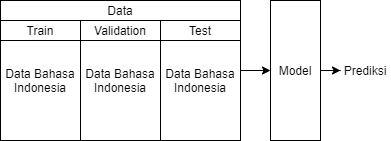
\includegraphics[width=0.75\textwidth]{resources/Data-tipe-A.png}
		\caption{Ilustrasi partisi data skenario monolingual}
		\label{fig:data_tipe_a}
	\end{figure}

	\subsection{Skenario Eksperimen}
	Terdapat tiga skenario eksperimen yang dilakukan untuk mencapai tujuan tugas akhir. Tiga skenario ini hanya memiliki perbedaan pada bahasa data yang digunakan untuk melakukan pelatihan. Berikut deskripsi tiap skenario:
	\begin{enumerate}
		\item \textbf{Skenario Monolingual}\\
		Dalam skenario ini, data untuk pelatihan, validasi, dan pengujian adalah data bahasa Indonesia. Skenario ini digunakan untuk menentukan \textit{baseline} dari performa model terhadap permasalahan. Detail ilustrasi dapat dilihat pada Gambar \ref{fig:data_tipe_a}.

		\begin{figure}[t]
		    \centering
		    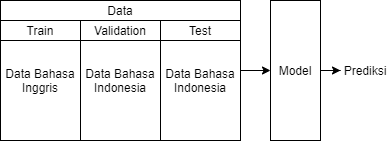
\includegraphics[width=0.75\textwidth]{resources/Data-tipe-B.png}
		    \caption{Ilustrasi partisi data skenario zero-shot}
		    \label{fig:data_tipe_b}
		\end{figure}

		\item \textbf{Skenario Zero-shot}\\
		Dalam skenario ini, data untuk pelatihan adalah data bahasa Inggris, sedangkan data validasi dan tes adalah data bahasa Indonesia. Skenario ini digunakan untuk melihat disparitas antara performa model yang dilatih dengan bahasa berbeda. Dari perbedaan performa skenario A dan B, representasi teks antar bahasa dari \textit{multilingual language model} dan juga hubungan antara dataset yang digunakan dapat dievaluasi. Detail ilustrasi dapat dilihat pada Gambar \ref{fig:data_tipe_b}.

		

		\begin{figure}[h]
		    \centering
		    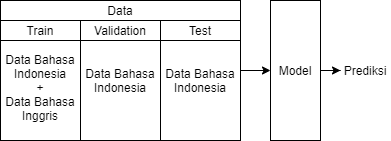
\includegraphics[width=0.75\textwidth]{resources/Data-tipe-C.png}
		    \caption{Ilustrasi partisi data skenario multilingual learning}
		    \label{fig:data_tipe_c}
		\end{figure}

		\item \textbf{Skenario Multilingual Learning}\\
		Dalam skenario ini, data untuk pelatihan adalah data bahasa Inggris dan Indonesia, sedangkan data validasi dan tes adalah data bahasa Indonesia. Pada skenario ini, perbandingan antara banyak data bahasa Inggris dengan data bahasa Indonesia divariasikan. Skenario ini digunakan untuk melihat seberapa efektif \textit{multilingual learning} dengan \textit{multilingual language model} pada klasifikasi teks bahasa Indonesia. Detail ilustrasi dapat dilihat pada Gambar \ref{fig:data_tipe_c}.
		
		
	\end{enumerate}


	
    \chapter{Eksperimen dan Pembangunan Sistem}

\section{Lingkungan Eksperimen dan Pembangunan Sistem}

Eksperimen dilakukan di platform \href{https://www.kaggle.com}{Kaggle} dengan Kernel gratisnya. Bahasa Pemrograman yang digunakan adalah bahasa Python versi 3.6.6. Pada \textit{fine-tuning} layer terakhir digunakan CPU 1xSingle core hyper threaded Xeon Processors @2.3Ghz, 46MB Cache. Pada \textit{fine-tuning} penuh digunakan TPU v3-8. Eksperimen dikembangkan menggunakan kombinasi pustaka PyTorch \parencite{paszke2017automatic} dan TensorFlow \parencite{tensorflow2015}.

Untuk memastikan bahwasanya eksperimen \textit{reproducible} dan tidak memiliki faktor acak, semua opsi \textit{seed} baik di System, Python, hingga pustaka Pytorch ditetapkan agar hasil tidak berubah jika eksperimen dijalankan berkali-kali dengan kondisi yang sama.

\begin{lstlisting}[language=Python]
def set_seed():
    seed=1
    random.seed(seed)
    torch.manual_seed(seed)
    torch.cuda.manual_seed_all(seed)
    np.random.seed(seed)
    os.environ['PYTHONHASHSEED'] = str(seed)
    torch.backends.cudnn.deterministic = True
\end{lstlisting}


\section{Eksperimen}
Eksperimen akan dilakukan dengan 2 model multilingual (XLM-R \& Multilingual BERT). Pada tiap eksperimen akan dilakukan variasi total data (500 / 1000 / 2500 / 5000 / 7500 / MAX) dan kelipatan bahasa asing pada skenario 3. Untuk konfigurasi model, callback berupa EarlyStopping dan ReduceLROnPlateau. Penggunaan callback EarlyStopping digunakanagar model tidak overfit. Sedangkan callback ReduceLROnPlateau digunakan untuk membantu model mencapai performa yang lebih baik. Semua eksperimen dijalankan hingga diberhentikan oleh callback EarlyStopping.


    \subsection{Hasil fine-tune layer terakhir}
        Berikut hasil eksperimen dengan model XLM-R: 
        \begin{enumerate}
            \item Analisis sentimen dengan data Prosa \\
            \begin{figure}[ht]
                \centering
                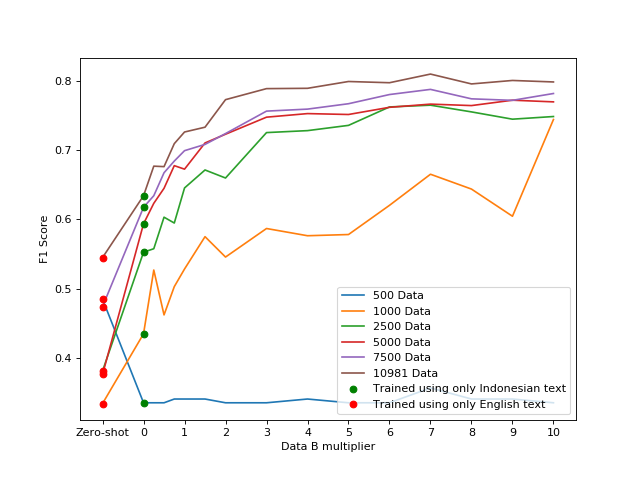
\includegraphics[width=0.75\textwidth]{resources/plot-head-prosa-xlmr.png}
                \caption{Plot antara F1-score dan kelipatan data bahasa Inggris pada berbagai total data di eksperimen data Prosa dengan model XLM-R.}
                \label{fig:plot_head_prosa_xlmr}
            \end{figure}
            Dapat dilihat pada Gambar \ref{fig:plot_head_prosa_xlmr}, performa analisis sentimen dataset Prosa sangat terbantu dengan penambahan data berbahasa Inggris. Di berbagai total data, penambahan bahasa Inggris menambah rata-rata F1-score sebesar 0.229. Penambahan performa terbesar diobservasi pada eksperimen dengan jumlah data yang sedikit. Performa model meningkat dari 0.734 pada skenario monolingual hingga mencapai 0.819 pada penambahan bahasa Inggris sebanya 7 kali lipat dari total bahasa Indonesianya.

            \item Analisis sentimen dengan data Trip Advisor \\
            \begin{figure}[ht]
                \centering
                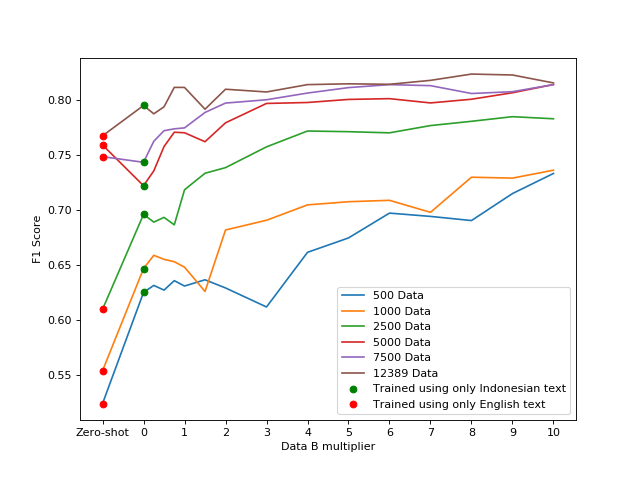
\includegraphics[width=0.75\textwidth]{resources/plot-head-trip-xlmr.png}
                \caption{Plot antara F1-score dan kelipatan data bahasa Inggris pada berbagai total data di eksperimen data Trip Advisor dengan model XLM-R.}
                \label{fig:plot_head_trip_xlmr}
            \end{figure}
            Dapat dilihat pada Gambar \ref{fig:plot_head_trip_xlmr}, performa analisis sentimen dataset Trip Advisor terbantu dengan penambahan data berbahasa Inggris. Di berbagai total data, penambahan bahasa Inggris menambah rata-rata F1-score sebesar 0.107. Penambahan performa terbesar juga diobservasi pada eksperimen dengan jumlah data yang sedikit. Performa model meningkat dari 0.794 pada skenario monolingual hingga mencapai 0.823 pada penambahan bahasa Inggris sebanya 8 kali lipat dari total bahasa Indonesianya.

            \item Klasifikasi ujaran kebencian \& kasar \\
            \begin{figure}[ht]
                \centering
                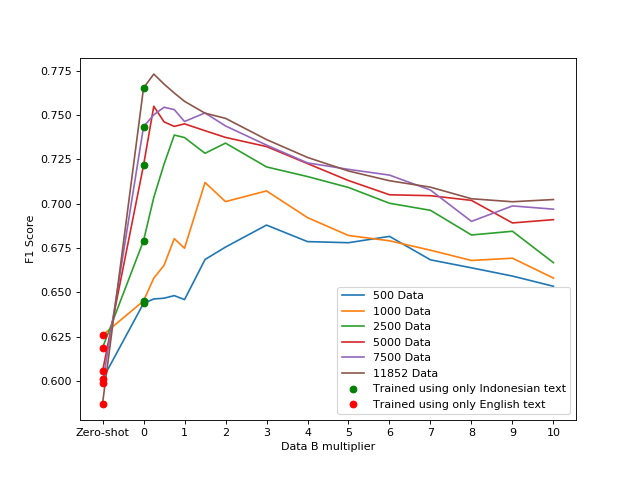
\includegraphics[width=0.75\textwidth]{resources/plot-head-toxic-xlmr.png}
                \caption{Plot antara F1-score dan kelipatan data bahasa Inggris pada berbagai total data di eksperimen klasifikasi ujaran kebencian dengan model XLM-R.}
                \label{fig:plot_head_toxic_xlmr}
            \end{figure}
            Dapat dilihat pada Gambar \ref{fig:plot_head_toxic_xlmr}, performa klasifikasi ujaran kebencian tidak terlalu terbantu dengan penambahan data berbahasa Inggris. Meski performa model sempat terbantu, penambahan lebih banyak data bahasa Inggris menurunkan performa model.

        \end{enumerate}
        
        Melalui rangkaian eksperimen dengan model XLM-R di atas, dapat dilihat korelasi antara perbedaan performa skenario \textit{zero-shot} dan \textit{monolingual} dengan performa skenario \textit{multilingual learning}. Eksperimen sentimen analisis Prosa memiliki rata-rata perbedaan skenario 1 dan 2 sebesar 0.0005. Dengan perbedaan yang sangat kecil, penambahan bahasa Inggris sangat bermanfaat. Eksperimen sentimen analisis Trip Advisor memiliki rata-rata perbedaan skenario 1 dan 2 sebesar 0.044. Dengan perbedaan yang cukup besar, penambahan bahasa Inggris menjadi berkurang manfaatnya. Terakhir, eksperimen klasifikasi ujaran kebencian memiliki perbedaan skenario 1 dan 2 sebesar 0.093. Dengan perbedaan yang sangat besar, penambahan bahasa Inggris menjadi kurang bermanfaat dan bahkan menurunkan performa model.

        Berikut hasil eksperimen dengan model mBERT: 

        \begin{figure}[ht]
            \minipage{0.5\textwidth}
              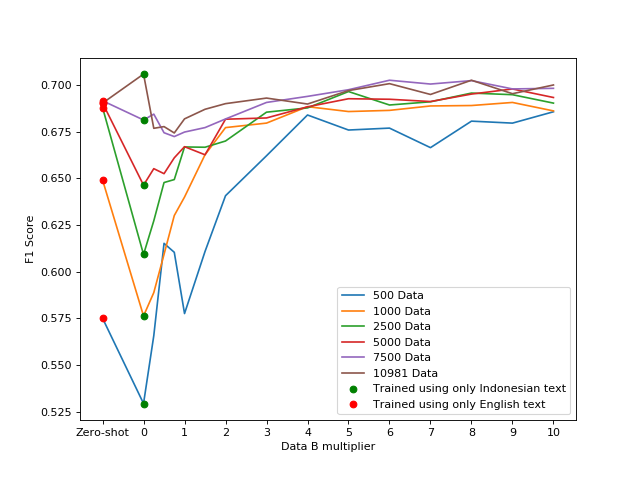
\includegraphics[width=\linewidth]{resources/plot-head-prosa-mbert.png}
              \caption{Plot Prosa model mBERT}\label{fig:plot_head_prosa_mbert}
            \endminipage\hfill
            \minipage{0.5\textwidth}
              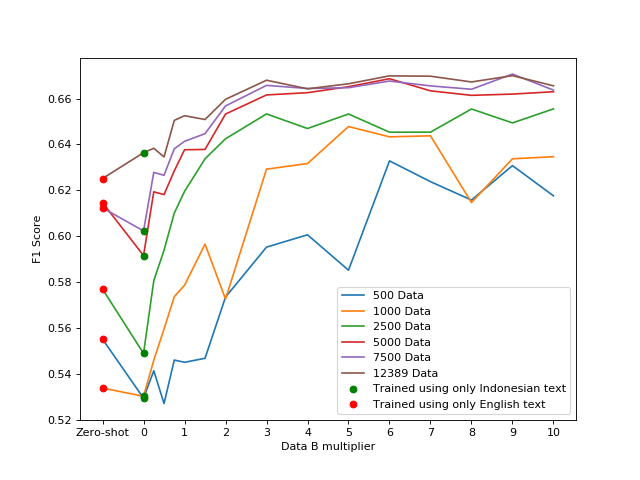
\includegraphics[width=\linewidth]{resources/plot-head-trip-mbert.png}
              \caption{Plot Trip model mBERT.}\label{fig:plot_head_trip_mbert}
            \endminipage
        \end{figure}

        \begin{figure}[ht]
            \centering
            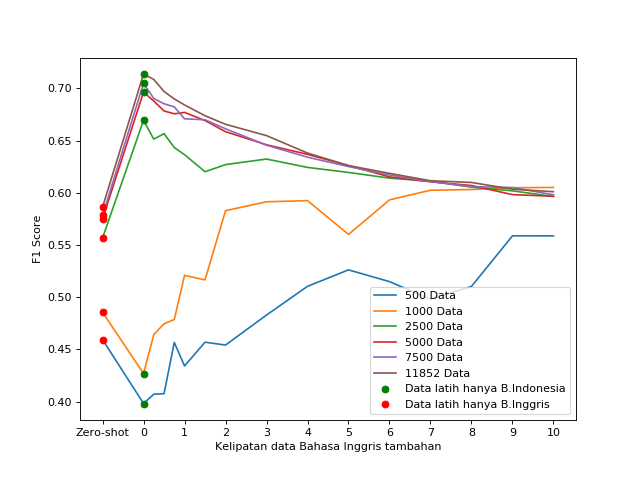
\includegraphics[width=0.5\textwidth]{resources/plot-head-toxic-mbert.png}
            \caption{Plot ujaran kebencian model mBERT.}\label{fig:plot_head_toxic_mbert}
        \end{figure}

        Melalui rangkaian eksperimen dengan model mBERT di atas, dapat dilihat hal yang sama dengan eksperimen model XLM-R. Secara umum performa mBERT lebih lemah dibanding XLM-R. Selain itu, dapat kita lihat juga biasnya \textit{pretraining} mBERT ke bahasa Inggris. Di berbagai total data, performa \textit{zero-shot} lebih bagus dibanding pasangan \textit{monolingual}-nya. Hal ini dikarenakan dalam pelatihan mBERT memiliki jumlah data bahasa Inggris yang tidak proporsional dengan data lainnya. Berbeda dengan XLM-R yang melakukan \textit{sampling} pada tiap \textit{batch} pelatihannya untuk memastikan performa model proporsional antar bahasa.
            

    \subsection{Hasil fine-tune penuh}
        Berikut hasil eksperimen dengan model XLM-R pada analisis sentimen Prosa dan klasifikasi ujaran kebencian :

        \begin{figure}[ht]
            \minipage{0.5\textwidth}
              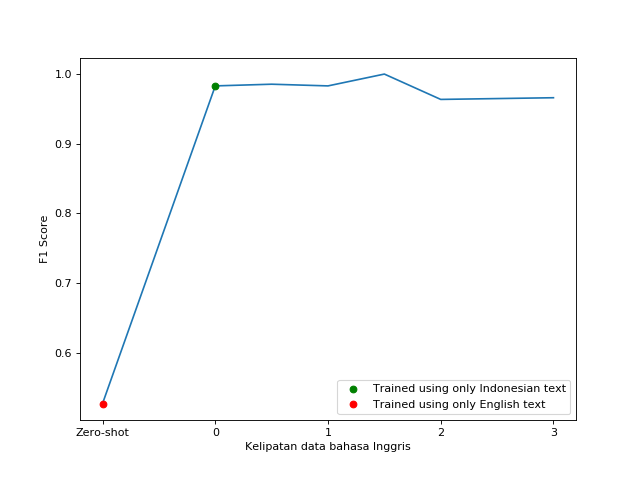
\includegraphics[width=\linewidth]{resources/plot-full-prosa-xlmr.png}
              \caption{Plot Prosa model XLM-R}\label{fig:plot_full_prosa_xlmr}
            \endminipage\hfill
            \minipage{0.5\textwidth}
              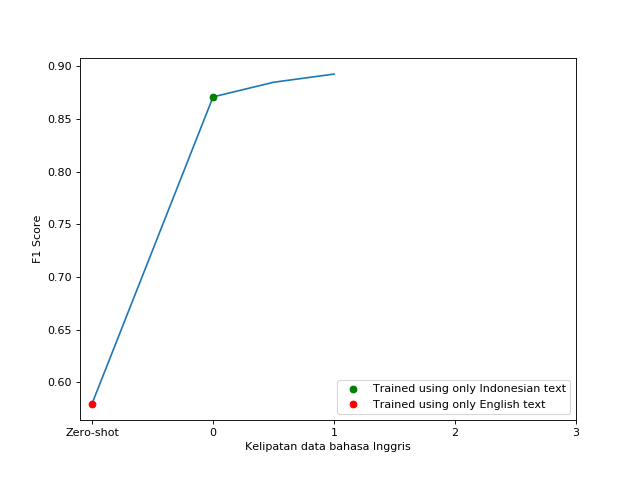
\includegraphics[width=\linewidth]{resources/plot-full-toxic-xlmr.png}
              \caption{Plot Ujaran kebencian model XLM-R.}\label{fig:plot_full_toxic_xlmr}
            \endminipage
        \end{figure}
        
        (baru sebagian eksperimen yang selesai dijalankan, plot di atas menggunakan seluruh data)
        
        Melalui sedikit eksperimen dengan model XLM-R di atas, dapat dilihat performa model XLM-R sangat bagus. Pada analisis sentimen dataset Prosa model berhasil memprediksi seluruh data tes dengan sempurna di skenario 3 dengan kelipatan bahasa Inggris 1.5. Pada klasifikasi ujaran kebencian model berhasil mencapai F1-Score 0.892 di skenario 3 dengan kelipatan bahasa Inggris 1.

    \subsection{Analisis hasil}
        

    \chapter{Kesimpulan dan Saran}

\section{Kesimpulan}
Berikut beberapa kesimpulan yang dapat ditarik dari tugas akhir ini:
\begin{enumerate}
    \item Penambahan dataset bahasa Inggris, terutama jika data bahasa Indonesia sedikit, dapat membantu meningkatkan performa klasifikasi teks bahasa Indonesia menggunakan \textit{multilingual language model}. Hanya saja, disparitas antara data bahasa Indonesia dengan data bahasa Inggris, yang dapat dilihat dari performa \textit{zero-shot} dan \textit{monolingual baseline}-nya, harus diperhatikan. Pada kasus analisis sentimen dengan dataset Prosa dan Trip Advisor, jarak tersebut masing-masing rata-rata 0.0005 dan 0.044. Sehingga eksperimen sentimen analisis skenario 3 pada data tersebut mendapat peningkatan F1-score masing-masing rata-rata 0.229 dan 0.107. Sedangkan pada klasifikasi ujaran kebencian yang jaraknya 0.093, penambahan data bahasa Inggris menjadi kurang bermanfaat dan bahkan menurunkan performa model.
    \item Penggunaan \textit{multilingual language model} yang di \textit{fine-tune} sepenuhnya sangat mangkus dalam klasifikasi teks bahasa Indonesia. Pada eksperimen sentimen analisis dataset Prosa, model ini mendapatkan F1-score sempurna. Sebuah peningkatan absolut dari penelitian sebelumnya yang mendapatkan F1-score 0,9369. Pada eksperimen klasifikasi ujaran kebencian, model ini mendapatkan F1-score 0,892 dan akurasi 89.4\%. Penelitian sebelumnya yang menggunakan 3 label, bukan yang disimplifikasi menjadi 2 seperti di penelitian ini, mendapatkan average accuracy tertinggi 77.36\%. Meski tidak dapat dibandingkan langsung dengan eksperimen terdekat penelitian sebelumnya, peningkatan ini tetap signifikan. 

\end{enumerate}

\section{Saran}
Berikut beberapa saran yang dapat ditarik dari tugas akhir ini:
\begin{enumerate}
    \item Terdapatnya disparitas antara dataset dapat menyebabkan turunnya performa. Untuk penelitian selanjutnya, dapat dicoba beberapa cara untuk mengatasi hal ini. Beberapa diantaranya adalah seperti penelitian \parencite{Lai_Oguz_Yang_Stoyanov_2019} yang menggunakan \textit{universal data augmentation} untuk mengurangi jarak tadi.
\end{enumerate}
    %----------------------------------------------------------------%

    % Daftar pustaka
    \printbibliography[title={Daftar Pustaka}]

    % Index
    \appendix

    \addcontentsline{toc}{part}{Lampiran}
    \part*{Lampiran}

    \chapter{Algoritma \textit{Byte Pair Encoding} Sederhana}
\label{appendix:simple_bpe_algorithm}

Algoritma (contoh nama file: \(bpe.py\)):
\begin{lstlisting}[language=Python]
import re, collections
def get_stats(vocab):
    pairs = collections.defaultdict(int)
    for word, freq in vocab.items():
        symbols = word.split()
        for i in range(len(symbols)-1):
            pairs[symbols[i],symbols[i+1]] += freq
    return pairs

def merge_vocab(pair, v_in):
    v_out = {}
    bigram = re.escape(' '.join(pair))
    p = re.compile(r'(?<!\S)' + bigram + r'(?!\S)')
    for word in v_in:
        w_out = p.sub(''.join(pair), word)
        v_out[w_out] = v_in[word]
    return v_out

vocab = {'l o w </w>' : 5, 'l o w e r </w>' : 2,
'n e w e s t </w>':6, 'w i d e s t </w>':3}
vocab_test = {'l o w e s t </w>': 1}

num_merges = 10
for i in range(num_merges):
    pairs = get_stats(vocab)
    best = max(pairs, key=pairs.get)
    print('~~~')
    vocab = merge_vocab(best, vocab)
    vocab_test = merge_vocab(best, vocab_test)
    print("best: ", best)
    print("vocab: ", vocab)
    print("vocab_test: ", vocab_test)
\end{lstlisting}

Setelah dijalankan di mesin bersistem operasi Ubuntu 18.04 dengan perintah
\begin{lstlisting}[language=bash]
    $ python3 bpe.py
\end{lstlisting}

akan didapatkan keluaran sebagai berikut:
\begin{lstlisting}[language=bash]
~~~
best:  ('e', 's')
vocab:  {'l o w </w>': 5, 'l o w e r </w>': 2, 'n e w es t </w>': 6, 'w i d es t </w>': 3}
vocab_test:  {'l o w es t </w>': 1}
~~~
best:  ('es', 't')
vocab:  {'l o w </w>': 5, 'l o w e r </w>': 2, 'n e w est </w>': 6, 'w i d est </w>': 3}
vocab_test:  {'l o w est </w>': 1}
~~~
best:  ('est', '</w>')
vocab:  {'l o w </w>': 5, 'l o w e r </w>': 2, 'n e w est</w>': 6, 'w i d est</w>': 3}
vocab_test:  {'l o w est</w>': 1}
~~~
best:  ('l', 'o')
vocab:  {'lo w </w>': 5, 'lo w e r </w>': 2, 'n e w est</w>': 6, 'w i d est</w>': 3}
vocab_test:  {'lo w est</w>': 1}
~~~
best:  ('lo', 'w')
vocab:  {'low </w>': 5, 'low e r </w>': 2, 'n e w est</w>': 6, 'w i d est</w>': 3}
vocab_test:  {'low est</w>': 1}
~~~
best:  ('n', 'e')
vocab:  {'low </w>': 5, 'low e r </w>': 2, 'ne w est</w>': 6, 'w i d est</w>': 3}
vocab_test:  {'low est</w>': 1}
~~~
best:  ('ne', 'w')
vocab:  {'low </w>': 5, 'low e r </w>': 2, 'new est</w>': 6, 'w i d est</w>': 3}
vocab_test:  {'low est</w>': 1}
~~~
best:  ('new', 'est</w>')
vocab:  {'low </w>': 5, 'low e r </w>': 2, 'newest</w>': 6, 'w i d est</w>': 3}
vocab_test:  {'low est</w>': 1}
~~~
best:  ('low', '</w>')
vocab:  {'low</w>': 5, 'low e r </w>': 2, 'newest</w>': 6, 'w i d est</w>': 3}
vocab_test:  {'low est</w>': 1}
~~~
best:  ('w', 'i')
vocab:  {'low</w>': 5, 'low e r </w>': 2, 'newest</w>': 6, 'wi d est</w>': 3}
vocab_test:  {'low est</w>': 1}
\end{lstlisting}
    % \chapter{Rincian Kasus Uji}

\end{document}
